\documentclass[a4paper,twoside]{book}

\usepackage[utf8]{inputenc}
\usepackage[english,russian]{babel}
\usepackage{fontspec}
\setmainfont{Liberation Serif}
\setmonofont{Liberation Mono}

\usepackage{graphicx}
\renewcommand{\thefigure}{\thesection.\arabic{figure}}
\usepackage{hyperref}
\usepackage{multirow}
\usepackage[absolute,overlay,showboxes]{textpos}
\usepackage{etoolbox}
\usepackage{longtable}
\usepackage{tikz}
\usepackage{lilyglyphs}
\usepackage{tabularx}
\usepackage{pgfplots}
\usepackage{circuitikz}

\usepackage{svg}

\urlstyle{same}
\usepackage[printonlyused,withpage]{acronym}

\graphicspath{ {images/} {../images/} }

%% This procedure adds the "Example" block to the text.
\newcommand{\example}[1]{
  \vspace{8pt}
  \begin{tabularx}{\textwidth}{m{1cm} m{9cm}}
    \includesvg[width=1.25cm]{the-noun-project/request-mirrored}
    & \textbf{Пример:} #1 \\
  \end{tabularx}
}

%% This procedure adds the "Experiment" block to the text.
\newcommand{\experiment}[2]{
  \vspace{8pt}
  \begin{tabularx}{\textwidth}{m{1cm} m{9cm}}
    \includesvg[width=1cm]{the-noun-project/flask}
    & \textbf{Эксперимент №#1:} #2 \\
  \end{tabularx}
}

\newcommand{\note}[1]{
  \vspace{8pt}
  \begin{tabularx}{\textwidth}{m{1cm} m{9cm}}
    \includesvg[width=1cm]{the-noun-project/note}
    & \textbf{Примечание:} #1 \\
  \end{tabularx}
}

\newcommand{\hotkey}[1]{
  \texttt{#1}
}

%% This procedure allows to insert a music note.
%% Syntax:
%%   \musicnote{<octave>}{<note-name>}{<frequency>}
\newcommand{\musicnote}[3]{
  &
  \ifstrequal{#2}{C}{До   & C#1}{}
  \ifstrequal{#2}{D}{Ре   & D#1}{}
  \ifstrequal{#2}{E}{Ми   & E#1}{}
  \ifstrequal{#2}{F}{Фа   & F#1}{}
  \ifstrequal{#2}{G}{Соль & G#1}{}
  \ifstrequal{#2}{A}{Ля   & A#1}{}
  \ifstrequal{#2}{B}{Си   & B#1 (H#1)}{}
  & #3 \\
}

\title{Автомато-программато-компарадио-кружок}
\author{Артём ``avp'' Попцов}
\date{\today}

\begin{document}

\maketitle

\tableofcontents

%%%%%%%%%%%%%%%%%%%%%%%%%%%%%%%%%%%%%%%%%%%%%%%%%%%%%%%%%%%%%%%%%%%%%%%%%%%%%%%%
\chapter*{Вступление}

%%%%%%%%%%%%%%%%%%%%%%%%%%%%%%%%%%%%%%%%%%%%%%%%%%%%%%%%%%%%%%%%%%%%%%%%%%%%%%%%
\section{Для кого предназначена данная книга?}
Дорогой читатель, добро пожаловать в наш уютный кружок технического творчества.
Здесь мы учимся работать со звуком, светом, электричеством, используя наши
знания для создания неожиданных, интересных и практически полезных проектов.  Мы
постараемся сделать ваш путь в мир электроники и программирования как можно
более интересным и лёгким.  Но и на вас лежит определённая отвественность --
во-первых, без вашего активного участия наши усилия могут не дать желаемого
эффекта.  Во-вторых, мы учимся вместе с вами, и ты, уважаемый читатель,
являешься активным участником работы над этой книгой.  Если найдёшь ошибки или
опечатки, не стесняйся писать нам по указанным в книге контактам -- мы
постараемся всё исправить в следующей версии книги.

Надеемся, что данная книга станет на какое-то время вашей настольной (или хотя
бы \emph{около-стольной}, но во всяком случе не \emph{под-стольной}) книгой,
которая поможет постичь искусство программирования и отчасти исследовать и
понять мир вокруг нас немного лучше, чем вы понимали прежде.

\section{Авторы}
В разработке данной книги принимали участие следующие люди:
\begin{itemize}
\item Денис Киселёв -- вклад в разработку отдельных глав книги; вычитка текста,
  участие в разработке и тестирование примеров, приведённых в книге.
\item Сергей Ермейкин -- вычитка текста, исправление ошибок.
\item Илья Маштаков – вычитка и доработка текста.
\end{itemize}

\section{Лицензия}
Copyright © 2016-2022 Артём ``avp'' Попцов.

Права на копирование сторонних изображений и материалов, использованных в данной
работе, принадлежат их владельцам.

Данная работа распространяется на условиях лицензии «Attribution-ShareAlike»
(«Атрибуция-СохранениеУсловий») 4.0 Всемирная (CC BY-SA 4.0)
\url{https://creativecommons.org/licenses/by-sa/4.0/deed.ru}

%%%%%%%%%%%%%%%%%%%%%%%%%%%%%%%%%%%%%%%%%%%%%%%%%%%%%%%%%%%%%%%%%%%%%%%%%%%%%%%%
\chapter{Основные принципы электротехники}

В первую очередь нам с вами надо рассмотреть базовые принципы того, как работает
электроника, чтобы впоследствии уметь собирать простые схемы.

Начнём с рассмотрения условий, которые необходимо выполнить, чтобы через
электрическую цепь шёл ток.

%%%%%%%%%%%%%%%%%%%%%%%%%%%%%%%%%%%%%%%%%%%%%%%%%%%%%%%%%%%%%%%%%%%%%%%%%%%%%%%%
\section{Напряжение}

Представим, что у нас есть некоторая ёмкость с водой (см. рисунок
\ref{fig:electronics-current-0}.)

\begin{figure}[ht]
  \centering
  \begin{tikzpicture}[
      declare function={f1(\x) = 0.15 * sin(8.0 * deg(\x));
    }]

    \draw[thick] (0, 0) -- (0, 4);
    \draw[thick] (2, 0) -- (2, 4);
    \draw[thick] (0, 0) -- (2, 0);

    \begin{scope}[yshift=3cm, color=blue]
      \draw (0, 0) plot[domain=0:2, variable=\x, samples=200, smooth] ({\x}, {f1(\x)});
    \end{scope}

  \end{tikzpicture}
  \caption{Пример ёмкости с водой.}
  \label{fig:electronics-current-0}
\end{figure}

Вода в ёмкости имеет некоторую \emph{потенциальную энергию}, которая может быть
потрачена с какой-либо целью.  Например, если мы внизу ведра проделаем
отверстие, то вода из него будет вытекать
(см. рис. \ref{fig:electronics-current-1}); если при этом под струю воды
подставить водяное колесо, то таким образом можно приводить в движение
механизмы.

\begin{figure}[ht]
  \centering
  \begin{tikzpicture}[
      declare function={f1(\x) = 0.15 * sin(8.0 * deg(\x));
    }]

    \draw[thick] (0, 0) -- (0, 4);
    \draw[thick] (2, 0.5) -- (2, 4);
    \draw[thick] (0, 0) -- (2, 0);

    \draw[thick, color=blue] (1, 1) -- (1, 0.25);
    \draw[thick, color=blue] (1, 0.25) -- (3, 0.25);
    \draw[thick, color=blue, ->] (3, 0.25) -- (3, -0.25);

    \begin{scope}[yshift=3cm, color=blue]
      \draw (0, 0) plot[domain=0:2, variable=\x, samples=200, smooth] ({\x}, {f1(\x)});
    \end{scope}

  \end{tikzpicture}
  \caption{Пример ёмкости с водой и отверстием снизу.}
  \label{fig:electronics-current-1}
\end{figure}

Проводя аналогию с электричеством можно сказать, что ёмкость имеет некоторое
\emph{напряжение} воды.  В электрической батарее как правило запасена
\emph{химическая энергия}, которая может быть высвобождена при определённых
условиях.

Напряжение в электрической цепи измеряется в \emph{Вольтах} (В).

Таким образом, мы можем сделать первый вывод: для протекания тока необходим
некий источник тока, обладающий некоторым напряжением.

%%%%%%%%%%%%%%%%%%%%%%%%%%%%%%%%%%%%%%%%%%%%%%%%%%%%%%%%%%%%%%%%%%%%%%%%%%%%%%%%
\section{Электрическая цепь}

Представим теперь две ёмкости, в одном из которой десять литров воды, в другой
-- ноль литров (или, как говорят люди, оно пустое), как показано рисунке
\ref{fig:electronics-circuits-0}.

\begin{figure}[ht]
  \centering
  \begin{tikzpicture}[
      declare function={f1(\x) = 0.15 * sin(8.0 * deg(\x));
    }]

    \draw[thick] (0, 0) -- (0, 4);
    \draw[thick] (2, 0) -- (2, 4);
    \draw[thick] (0, 0) -- (2, 0);

    \draw[thick] (3, 0) -- (3, 4);
    \draw[thick] (5, 0) -- (5, 4);
    \draw[thick] (3, 0) -- (5, 0);

    \begin{scope}[yshift=3cm, color=blue]
      \draw (0, 0) plot[domain=0:2, variable=\x, samples=200, smooth] ({\x}, {f1(\x)});
    \end{scope}

    \draw (1, 0) node[below] {А};
    \draw (4, 0) node[below] {Б};

  \end{tikzpicture}
  \caption{Пример двух ёмкостей: с водой (А) и пустая (Б).}
  \label{fig:electronics-circuits-0}
\end{figure}

Если мы соединим ёмкость ``А'' и ``Б'' трубой, то вода потечёт из ``А'' в ``Б'',
по законам физики (см. рисунок \ref{fig:electronics-circuits-1}.)

\begin{figure}[ht]
  \centering
  \begin{tikzpicture}[
      declare function={f1(\x) = 0.15 * sin(8.0 * deg(\x));
    }]

    \draw[thick] (0, 0) -- (0, 4);
    \draw[thick] (2, 0.5) -- (2, 4);
    \draw[thick] (0, 0) -- (2, 0);

    \draw[thick] (3, 0.5) -- (3, 4);
    \draw[thick] (5, 0) -- (5, 4);
    \draw[thick] (3, 0) -- (5, 0);

    \draw[thick] (2, 0) -- (3, 0);
    \draw[thick] (2, 0.5) -- (3, 0.5);

    \draw[thick, color=blue, ->] (1, 0.25) -- (4, 0.25);


    \begin{scope}[yshift=3cm, color=blue]
      \draw (0, 0) plot[domain=0:2, variable=\x, samples=200, smooth] ({\x}, {f1(\x)});
    \end{scope}

    \draw (1, 0) node[below] {А};
    \draw (4, 0) node[below] {Б};

  \end{tikzpicture}
  \caption{Пример двух ёмкостей: с водой (А) и пустая (Б), соединённые трубкой.}
  \label{fig:electronics-circuits-1}
\end{figure}

Соединив две ёмкости, мы получили \emph{замкнутую цепь}, по которой возможен ток
воды.  Подобным образом работают электрические цепи, только вместо тока воды в
электрических цепях происходит ток элементарных заряженных частиц.

Итак, второе правило, которое мы должны усвоить: электрический ток возможен в
замкнутой цепи.

Ток в электрической цепи измеряется в \emph{Амперах} (А).

Электрическая схема, аналогичная по своей сути
рис. \ref{fig:electronics-circuits-1}, будет выглядеть, как на
рис. \ref{fig:electronics-simple-circuit}.

\begin{figure}[ht]
  \centering
  \begin{circuitikz}
    \draw (0,0)
    to[battery, l=Батарея] (0,2) % The voltage source
    to[short] (2,2)
    to[full led, l=Светодиод] (2,0) % The lamp
    to[short] (0,0);
  \end{circuitikz}
  \caption{Электрическая цепь с батареей в качестве источника тока и светодиодом
    в качестве нагрузки.}
  \label{fig:electronics-simple-circuit}
\end{figure}

\section{Разность потенциалов}

Посмотрим ещё раз на рис. \ref{fig:electronics-circuits-1}.  Вода перетекает из
ёмкости А в ёмкость Б по трубе.  Как только в уровни воды в ёмкостях сравняются,
то ток воды по трубе остановится (см. рис. \ref{fig:electronics-circuits-2}.)

\begin{figure}[ht]
  \centering
  \begin{tikzpicture}[
      declare function={f1(\x) = 0.15 * sin(8.0 * deg(\x));
    }]

    \draw[thick] (0, 0) -- (0, 4);
    \draw[thick] (2, 0.5) -- (2, 4);
    \draw[thick] (0, 0) -- (2, 0);

    \draw[thick] (3, 0.5) -- (3, 4);
    \draw[thick] (5, 0) -- (5, 4);
    \draw[thick] (3, 0) -- (5, 0);

    \draw[thick] (2, 0) -- (3, 0);
    \draw[thick] (2, 0.5) -- (3, 0.5);


    \begin{scope}[yshift=1.5cm, color=blue]
      \draw (0, 0) plot[domain=0:2, variable=\x, samples=200, smooth] ({\x}, {f1(\x)});
    \end{scope}

    \begin{scope}[yshift=1.5cm, xshift=3cm, color=blue]
      \draw (0, 0) plot[domain=0:2, variable=\x, samples=200, smooth] ({\x}, {f1(\x)});
    \end{scope}

    \draw (1, 0) node[below] {А};
    \draw (4, 0) node[below] {Б};

  \end{tikzpicture}
  \caption{Пример двух ёмкостей с равным уровнем воды.}
  \label{fig:electronics-circuits-2}
\end{figure}

Аналогом в электронике этой ситуации, когда ток перестаёт течь, является
разряженная батарейка: в процессе эксплуатации химические реакции, дающие
разность уровней -- или, как говорят в электронике, \emph{разность потенциалов}
-- в ней постепенно замедляются, вплоть до момента, когда батарейка больше не
может давать нужный ток.

Таким образом, вторым условием для электрического тока является наличие разности
потенциалов.

Интересным фактом является то, что для протекания электрического тока (как и
воды) не обязательно иметь разность потенциалов между каким-то положительным
значением и нулём.  Проводя опять же аналогию с водой, если мы возьмём две
соединённые ёмкости, стоящие на одном уровне но с разными уровнями жидкости, то
ток воды будет, пока уровни жидкости не сравняются в обоих ёмкостях
(см. рис. \ref{fig:electronics-circuits-3}.)

\begin{figure}[ht]
  \centering
  \begin{tikzpicture}[
      declare function={f1(\x) = 0.15 * sin(8.0 * deg(\x));
    }]

    \draw[thick] (0, 0) -- (0, 4);
    \draw[thick] (2, 0.5) -- (2, 4);
    \draw[thick] (0, 0) -- (2, 0);

    \draw[thick] (3, 0.5) -- (3, 4);
    \draw[thick] (5, 0) -- (5, 4);
    \draw[thick] (3, 0) -- (5, 0);

    \draw[thick] (2, 0) -- (3, 0);
    \draw[thick] (2, 0.5) -- (3, 0.5);

    \draw[thick, color=blue, ->] (1, 0.25) -- (4, 0.25);


    \begin{scope}[yshift=3cm, color=blue]
      \draw (0, 0) plot[domain=0:2, variable=\x, samples=200, smooth] ({\x}, {f1(\x)});
    \end{scope}

    \begin{scope}[yshift=1.5cm, xshift=3cm, color=blue]
      \draw (0, 0) plot[domain=0:2, variable=\x, samples=200, smooth] ({\x}, {f1(\x)});
    \end{scope}

    \draw (1, 0) node[below] {А};
    \draw (4, 0) node[below] {Б};

  \end{tikzpicture}
  \caption{Пример двух ёмкостей с разными уровнями воды, соединённые трубкой.}
  \label{fig:electronics-circuits-3}
\end{figure}

То же самое относится к ёмкостям, стоящим на разных уровнях.  В электронике для
протекания тока достаточная любая разность потенциалов; примерами разных
потенциалов могут быть 5В и 10В (где разность будет в 5В), или же -5В и +5В (что
даёт разницу в 10В.)

%%%%%%%%%%%%%%%%%%%%%%%%%%%%%%%%%%%%%%%%%%%%%%%%%%%%%%%%%%%%%%%%%%%%%%%%%%%%%%%%
\section{Сопротивление}

Чтобы понять, с какой скоростью вода будет перетекать из сосуда в сосуд,
необходимо знать параметры трубопровода, соединяющего их -- иными словами,
\emph{проводника воды}.  Основным параметром проводника является
\emph{сопротивление} -- чем выше этот параметр, тем медленне вода будет течь.

Примером проводника с высоким сопротивлением является трубопровод с малым
сечением (или диаметром) труб, как показано на
рис. \ref{fig:electronics-resistance-0}.

\begin{figure}[ht]
  \centering
  \def\offset{6}
  \begin{tikzpicture}[
      declare function={f1(\x) = 0.15 * sin(8.0 * deg(\x));
    }]

    \draw[thick] (0, 0) -- (0, 4);
    \draw[thick] (2, 0.5) -- (2, 4);
    \draw[thick] (0, 0) -- (2, 0);

    \draw[thick] (3, 0.5) -- (3, 4);
    \draw[thick] (5, 0) -- (5, 4);
    \draw[thick] (3, 0) -- (5, 0);

    \draw[thick] (2, 0) -- (3, 0);
    \draw[thick] (2, 0.5) -- (3, 0.5);

    \draw[thick] (\offset, 0) -- (\offset, 4);
    \draw[thick] (\offset + 2, 0.25) -- (\offset + 2, 4);
    \draw[thick] (\offset, 0) -- (\offset + 2, 0);

    \draw[thick] (\offset + 3, 0.25) -- (\offset + 3, 4);
    \draw[thick] (\offset + 5, 0) -- (\offset + 5, 4);
    \draw[thick] (\offset + 3, 0) -- (\offset + 5, 0);

    \draw[thick] (\offset + 2, 0) -- (\offset + 3, 0);
    \draw[thick] (\offset + 2, 0.25) -- (\offset + 3, 0.25);

    \draw[thick, color=blue, ->] (1, 0.25) -- (4, 0.25);

    \draw[thick, color=blue, ->] (\offset + 1.5, 0.125) -- (\offset + 3.5, 0.125);

    \begin{scope}[yshift=1.5cm, color=blue]
      \draw (0, 0) plot[domain=0:2, variable=\x, samples=200, smooth] ({\x}, {f1(\x)});
    \end{scope}

    \begin{scope}[yshift=1.5cm, xshift=6 cm, color=blue]
      \draw (0, 0) plot[domain=0:2, variable=\x, samples=200, smooth] ({\x}, {f1(\x)});
    \end{scope}

    \draw (1, 0) node[below] {А};
    \draw (4, 0) node[below] {Б};
    \draw (7, 0) node[below] {В};
    \draw (10, 0) node[below] {Г};

  \end{tikzpicture}
  \caption{Пример ёмкостей, соединённых трубами разных сопротивлений.}
  \label{fig:electronics-resistance-0}
\end{figure}

Уменьшение сечения трубы приводит к увеличению её сопротивления для тока воды.
Данное правило применимо также для электрических цепей, где сечение проводника
(провода) и его сопротивление имеют обратную зависимость: чем больше сечение,
тем меньше сопротивление; чем меньше сопротивление, тем больше ток.

Для наглядности предположим, что ёмкости ``В'' и ``Г'' на
рис. \ref{fig:electronics-resistance-0} соединены трубой с сечением вполовину от
того, что соединяет ёмкости ``А'' и ``Б''.  Тогда ток воды между ёмкостями ``В''
и ``Г'' будет в два раза меньше, чем между ёмкостями ``А'' и ``Б''.

В электронике сопротивление проводника измеряется в \emph{Омах} (англ. ``Ohm'').

Взаимосвязь тока, напряжения и сопротивления описывается \emph{законом Ома}.

Используя закон Ома, можно посчитать ток для электрической цепи по формуле
\ref{equation:elemctronics-ohms-law-0}.

\begin{equation}
  \mbox{I} = \frac{\mbox{U}}{\mbox{R}}
  \label{equation:elemctronics-ohms-law-0}
\end{equation}

Где ``I'' -- это сила тока (в Амперах), ``U'' -- это напряжение (в Вольтах), а
``R'' -- это сопротивление (в Омах).

Как можно видеть из данной формулы, увеличение сопротивления проводника в два
раза уменьшает ток, идущий по электрической цепи, в два раза.

\note{ Для запоминания закона Ома можно использовать детский стишок: ``Знает
  каждый пионер: сила тока -- U на R!''.  }

%%%%%%%%%%%%%%%%%%%%%%%%%%%%%%%%%%%%%%%%%%%%%%%%%%%%%%%%%%%%%%%%%%%%%%%%%%%%%%%%
\chapter{Знакомство с набором разработки Arduino}

\section{Введение}
По нашему мнению, программирование является двоякой дисциплиной: с одной
стороны, это – один из видов творчества, позволяющий человеку создать что-то
необычное, новое и, возможно, полезное для общества; с другой стороны, это –
инструмент, позволяющий решать практические, прикладные задачи. Как кисти и
краски художника, или инструменты музыканта, инструменты программиста имеют
большое разнообразие в видах и применениях. Чтобы освоить их в полной мере
требуются годы. Тем не менее, долгий путь начинается с первого шага.

Данная книга позволяет людям, желающим освоить программирование, сделать первый
шаг на пути в профессии программиста. Вам предлагается изучить основы
программирования на C, разрабатывая приложения для платформы Arduino.

\section{Работа с макетной платой}

Макетная плата позволяет собирать схемы (подключать электронику) без применения
пайки --- это упрощает прототипирование и ускоряет процесс разработки проектов.
Компоненты просто вставляются в слоты на макетной плате для соединения
(см. рис. \ref{fig:breadboard-led}.)

\begin{figure}[ht]
  \centering
  \caption{Пример подключения светодиода к Arduino Mega 2560 через макетную
    плату.}
  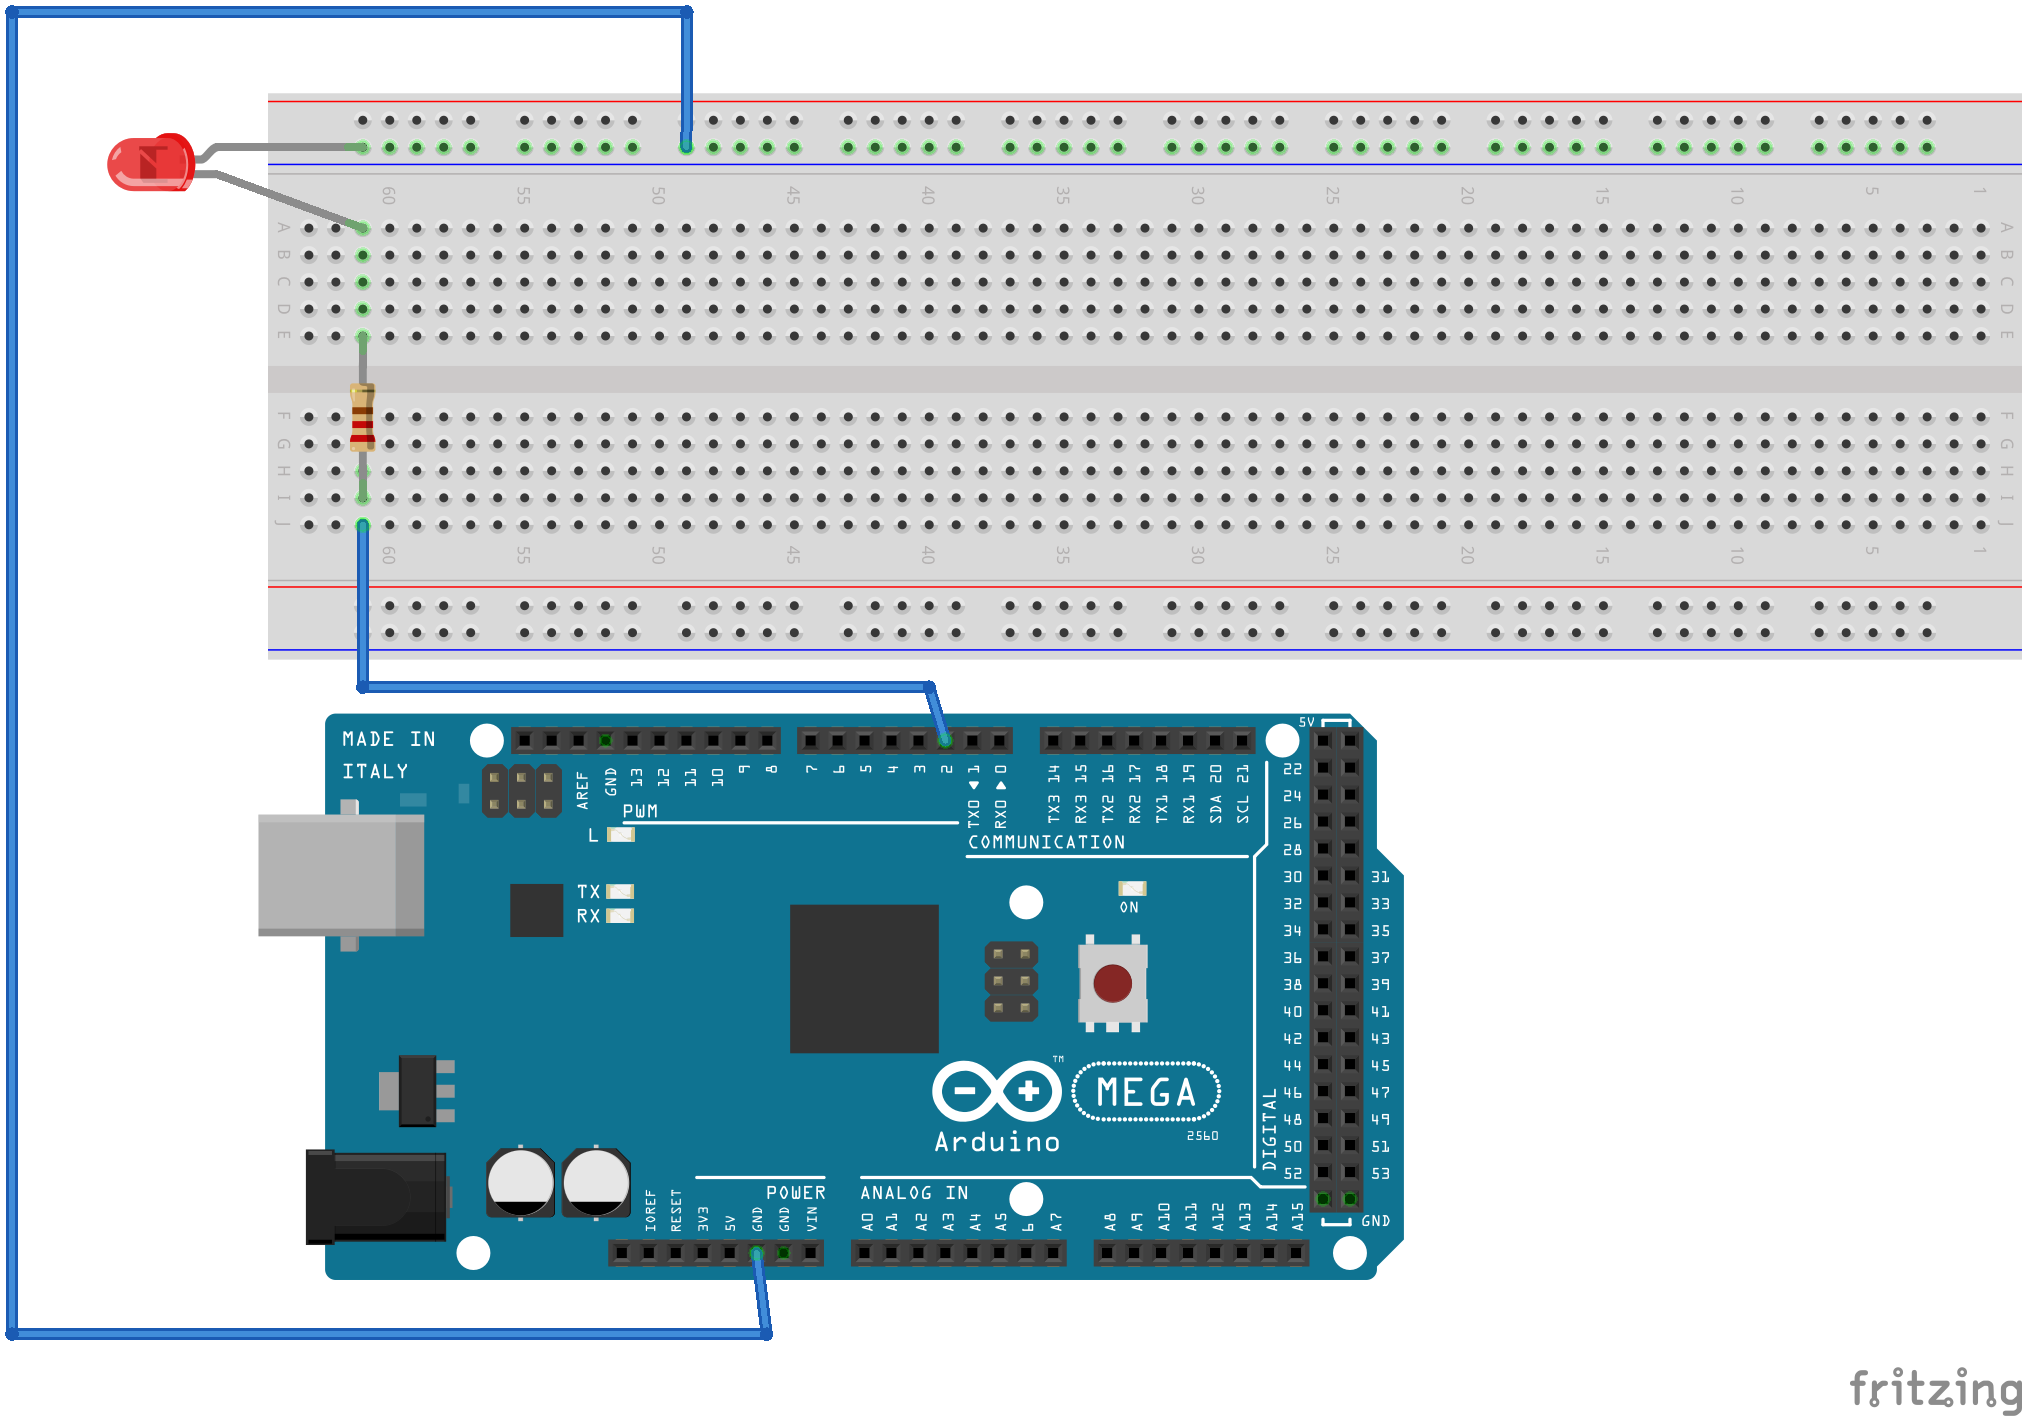
\includegraphics[width=12cm]{schematics/001-led}
  \label{fig:breadboard-led}
\end{figure}

\begin{itemize}
\item Черный провод подключен к arduino и идёт на вывод GND (минус)
\item Синий провод подключен к arduino и идёт на вывод 5V (плюс)
\end{itemize}

\note{ Обратите внимание, что светодиоды (и некоторые другие элементы)
  подключаются к платформе Arduino через резистор -- это необходимо для
  обеспечения бесперебойной работы схемы и предупреждения всяческих поломок и
  ухудшения работы как отдельных деталей, так и схемы в целом.  }

\section{Подключение Arduino к компьютеру}
Чтобы подключить ардуино к компьютеру вам потребуется сама платформа Arduino (в
нашем случае мы используем Arduino Mega 2560) и кабель стандарта USB-В.

Соедините Arduino с компьютером через USB-кабель. Вы увидите, как на плате
загорится светодиод ``ON''.

Теперь необходимо настроить Arduino IDE для работы с подключенной Arduino, для
этого нужно войти в панель ``Инструменты'' затем ``Плата'' -- в этом меню
выберите 6Arduino с которой вы сейчас работаете, затем в подменю ``Порт''
выберите порт, к которому подключена Arduino.

\section{Знакомство со средой разработки Arduino}
Среда разработки Arduino (Arduino IDE) состоит из встроенного текстового
редактора программного кода, области сообщений, окна вывода текста (консоли),
панели инструментов с кнопками часто используемых команд и нескольких меню. Для
загрузки программ и связи с компьютером среда разработки подключается к
аппаратной части Arduino.

Скачать среду разработки можно с официального сайта Arduino:
\url{https://www.arduino.cc/en/Main/Software}.

Перед скачиванием будет предложено пожертвовать денег проекту Arduino для
дальнейшего развития, но этот шаг необязателен и может быть выполнен на ваше
усмотрение.

Ниже приведено описание кнопок в интерфейсе Arduino IDE.

\begin{tabular}{p{4cm}|p{6cm}}
  Название & Описание \\
  \hline \hline
  Verify/Compile (Проверка) & Проверка программного кода. \\
  \hline
  Upload (Загрузка) & Компилирует программный код.\\
  \hline
  New (Создать) & Создание нового скетча.\\
  \hline
  Open (Открыть) & Открыть скетч.\\
  \hline
  Save (Сохранить) & Сохранить скетч.\\
  \hline
  Serial Monitor (Монитор порта) & Открыть монитор порта.\\
\end{tabular}

\section{Основы работы с мультиметром}
Мультиметр -- незаменимый прибор, с его помощью можно узнать сопротивление
резистора, измерить напряжение, произвести проверку на проводимость
(``прозвонка''), узнать цвет и полярность светодиода и многое другое.

Далее приведена таблица на которой отражены основные символы, встречающиеся на
корпусе прибора, необходимые для работы с мультиметром:

%%%%%%%%%%%%%%%%%%%%%%%%%%%%%%%%%%%%%%%%%%%%%%%%%%%%%%%%%%%%%%%%%%%%%%%%%%%%%%%%
\section{Структура программы на Arduino}

Программа для Arduino обычно состоит из двух основных частей, также называемых
функциями: "setup" и "loop". Пример программы, которая мигает одним светодиодом:
\begin{verbatim}
void setup() {
    pinMode(2, OUTPUT);
}

void loop() {
    digitalWrite(2, HIGH);
    delay(500);
    digitalWrite(2, LOW);
    delay(500);
}
\end{verbatim}

Функция \texttt{setup} производит инициализацию микроконтроллера при его
включении. В неё следует помещать все команды, которые должны выполняться
единожды на старте системы.

Цифровой порт (или, по-другому, пин) Arduino может находиться в двух состояниях.
В режиме входа пин считывает напряжение, а в режиме выхода – позволяет выдавать
на пине такое же напряжение.

Рассмотрим приведённый выше пример. В \texttt{setup} выполняется функция
\texttt{pinMode}, которая позволяет настроить режим работы указанного пина как
вход или выход:

\begin{verbatim}
  pinMode(pin, mode);
\end{verbatim}

где \texttt{pin} -- номер пина, \texttt{mode} -- режим работы
(\texttt{INPUT}/\texttt{OUTPUT}).

В \texttt{loop} вызываются две функции: \texttt{digitalWrite} и \texttt{delay}.

Функция
\begin{verbatim}
  digitalWrite(pin,value);
\end{verbatim}

где \texttt{pin} -– номер пина, \texttt{value} -- уровень сигнала
(\texttt{HIGH}/\texttt{LOW}), подаёт на пин высокое или низкое напряжение.

Функция
\begin{verbatim}
delay(value);
\end{verbatim}

где \texttt{value} -- количество миллисекунд, останавливает выполнение программы
на указанное время.

\subsection{Задачи}
\begin{itemize}
\item Соберите на макетной плате ``бегущий огонь'': светодиоды должны поочерёдно
  включаться и выключаться, один за другим.
\item Модифицируйте ``бегущий огонь'' так, чтобы он бежал сначала в одну
  сторону, затем в другую.
\end{itemize}

\section{Переменные и память}

\emph{Переменная} -- это ключевое понятие в программировании. Любая программа
работает с данными. Возьмём для наглядности некую программу- калькулятор,
умеющую складывать два числа. Чтобы микроконтроллер мог работать с этими числами
их нужно где-то хранить. Где? В оперативной памяти. Все данные, которые
используются микроконтроллером во время работы, хранятся именно там. Для работы
нашего калькулятора нужно загрузить в ячейки оперативной памяти два
числа-операнда, которые нужно сложить, например 15 и 3:

\begin{tabular}{p{4cm}|p{6cm}}
  Адрес ячейки & Значение ячейки \\
  \hline \hline
  0000 & 15 \\
  \hline
  0001 & 3 \\
  \hline
  0003 & 0 \\
  ... & ... \\
\end{tabular}

\emph{Переменная} -- это ячейка данных в оперативной памяти (ОЗУ). Объявить
переменную –- значит сказать компьютеру выделить какую-нибудь ячейку памяти для
наших нужд.

Переменная в языке С++ имеет определённый тип и уникальное имя. Объявление
(\emph{инициализация}) переменной выглядит следующим образом:

\begin{verbatim}
тип имя = значение;
\end{verbatim}

То есть, чтобы загрузить в оперативную память два числа 15 и 3, мы должны написать
следующее:

\begin{verbatim}
int a = 15;
int b = 3;
\end{verbatim}

Слово \texttt{int} это тип переменной, означает, что эта переменная является
числом.

Также следует объявить переменную для хранения результата сложения:

Дальше -- складываем значения двух переменных \texttt{a} и \texttt{b}:

\begin{verbatim}
int result = a + b;
\end{verbatim}

Здесь мы присвоили переменной \texttt{result} результат операции сложения двух
переменных.

\emph{ВАЖНО!} Имя переменной может состоять только из букв, цифр и нижнего
подчёркивания, причём имя не может начинаться с цифры.

Вернёмся к нашим светодиодам. Объявим новую переменную:

\begin{verbatim}
int k = 500;
\end{verbatim}

Что мы можем с ней сделать? Например, в программе мигания светодиодом заменим ею
значение задержки в функции \texttt{delay}. Вообще, переменным следует давать
осмысленные имена, в нашем случае пусть это будет не \texttt{k}, а
\texttt{delay\_val}:

\begin{verbatim}
void loop() {
    int delay_val = 500;
    digitalWrite(2, HIGH);
    delay(delay_val);
    digitalWrite(2, LOW);
    delay(delay_val);
}
\end{verbatim}

Таким образом, мы сможем поменять значения всех задержек одной заменой значения
\texttt{delay\_val}:

\begin{verbatim}
void loop() {
    int delayVal = 600;
    // ...
}
\end{verbatim}

Можно, например, увеличивать \texttt{delay\_val} на 100 при каждом выполнении
\texttt{loop}:

\begin{verbatim}
void loop() {
    int delay_val = 100;
    digitalWrite(2, HIGH);
    delay(delay_val);
    digitalWrite(2, LOW);
    delay(delay_val);
    delay_val = delay_val + 100;
}
\end{verbatim}

Кстати, строчку \texttt{delay\_val = delay\_val + 100} можно заменить на
\texttt{delay\_val += 100} и результат будет тем же, но запись короче.

\texttt{+=} -- оператор присваивания, совмещённый со сложением.

Существуют также другие операторы подобного рода -- например, ``-=''
(читается ``минус-равно'') Если мы запустим этот код, то увидим, что задержка
переключения светодиодов… не меняется. Почему? При каждом выполнении loop()
каждый раз объявляется новая переменная \texttt{delay\_val} со значением 100 и
потому задержка остаётся той же. Сейчас delayVal объявлена как локальная
переменная внутри \texttt{loop}, следует объявить её за пределами функции, чтобы
она стала глобальной:

\begin{verbatim}
int delay_val = 100;

void loop() {
  digitalWrite(2, HIGH);
  delay(delay_val);
  digitalWrite(2, LOW);
  delay(delay_val);

  delay_val += 100;
}
\end{verbatim}

Теперь всё будет работать. Но так задержка будет бесконтрольно расти. Решением
будет сделать так, чтобы \texttt{delay\_val} увеличивалась до какого-то
порогового значения, например, до 600. Для этого нужно добавить условие
(\texttt{if}):

\begin{verbatim}
int delay_val = 100;

void loop() {
    digitalWrite(2, HIGH);
    delay(delay_val);
    digitalWrite(2, LOW);
    delay(delay_val);

    if (delay_val < 600){
      delay_val += 100;
    }
}
\end{verbatim}

Об условиях и других управляющих конструкциях -- в следующей главе.

\chapter{Управляющие конструкции языка C++}

\section{Условия}

Иногда во время выполнения программы следует принять решение о том, что делать
дальше. Для того, чтобы компьютер мог сделать правильный выбор, по какому пути
пойти, нам, как программистам, следует описать условия в коде программы: если
условие выполняется, делаем одно, иначе -- делаем другое.

Условия в программах описываются при помощи специальных управляющих конструкций.
В языке C++ у нас есть две основные конструкции. Первая из них -- оператор
\texttt{if} (буквально в переводе с английского ``если''). Пример использования:

\begin{verbatim}
if (a > 10) {
    // действие, выполняемое, если значение
    // переменной 'a' больше 10.
}
\end{verbatim}

Если нужно проверить равно ли значение переменной чему-либо, используют оператор
сравнения ``=='':

\begin{verbatim}
if (a == 10) {
    // действие, выполняемое, если значение
    // переменной 'a' равно 10.
}
\end{verbatim}

Не путайте оператор сравнения ``=='' с оператором присваивания ``='' - это важно!

Часто необходимо не только делать что-либо при выполнении условия, но и
предоставить альтернативную инструкцию (или набор инструкций), выполняемую
тогда, когда условие не выполняется. В этом случае используют конструкцию
\texttt{if ... else}:

\begin{verbatim}
if (a > 10) {
  // действие, выполняемое, если значение
  // переменной 'a' больше 10.
} else {
  // действие, выполняемое, если значение
  // переменной 'a' меньше или равно 10.
}
\end{verbatim}

Второй оператор, который нам будет встречаться, это так называемый
\emph{оператор выбора} \texttt{switch}. С ним познакомимся позже. Он удобен,
например, тогда, когда нам нужно выполнять несколько разных действий в
зависимости от значения переменной, и этих действий много.

\section{Циклы}

Простые программы, вроде ``бегущего огня'', могут быть написаны простым
копированием и вставкой алгоритма мигания светодиода (возможно, с небольшими
модификациями).

А теперь представьте, что вам требуется запрограммировать ``бегущий огонь'' на
100 светодиодов. Утомительная задача, не правда ли? Для того, чтобы не делать
тупую работу по копированию одного и того же кода много раз, программистами
придуманы специальные управляющие конструкции, называемые \emph{циклами}.

Циклы бывают разные. Основные виды циклов, которые вам будут встречаться
практически в любом языке программирования:
\begin{itemize}
\item Цикл со счётчиком (также называемый ``параметрический цикл'').
\item Цикл с предусловием.
\item Цикл с постусловием.
\end{itemize}

Каждый вид циклов имеет собственную реализацию в языке программирования, который
мы используем (C++).

\subsection{Цикл со счётчиком}

Цикл со счётчиком реализуется конструкцией \texttt{for} -- она позволяет нам
создать счётчик, задать его начальное значение, описать условие выполнения цикла
и операцию изменения счётчика:

\begin{verbatim}
//                   5.
//        1.         2.           4.
for (int pin = 0; pin < 10; pin = pin + 1) {
    // 3. (тело цикла)
}
\end{verbatim}

Выполняется эта конструкция в следующем порядке:
\begin{enumerate}
\item объявляем переменную и присваиваем ей значение 0 (шаг 1);
\item переходим к проверке, где смотрим, выполняется ли условие (шаг 2);
\item после этого, если условие 2 выполняется, мы переходим к телу цикла (шаг 3);
\item после выполнения тела цикла, мы переходим к изменению значения счётчика (шаг 4);
\item после шага 4 мы опять возвращаемся к шагу 2, если условие выполняется, то
  переходим к шагу 3 и т.д.
\end{enumerate}

\subsection{Цикл с предусловием}

Другим распространённым видом цикла является цикл с предусловием, реализуемый в
С++ конструкцией \texttt{while} -- данный вид цикла удобен в тех случаях, когда
мы не знаем точного количества раз, сколько нужно повторить тело цикла (не знаем
количество итераций.)

Общий вид цикла \texttt{while} таков:
\begin{verbatim}
int pin = 2;

while (pin < 10) {
    // тело цикла
}
\end{verbatim}

\subsection{Цикл с постусловием}

Кроме вышеперечисленных видов циклов, есть ещё цикл с постусловием, где
проверка условия выполнения цикла осуществляется после выполнения тела цикла.
Реализуется данный вид циклов конструкцией \texttt{do..while}.

Он достаточно редкоиспользуется и мы не будем на нём здесь останавливаться.

\subsection{Зачем столько видов циклов?}

Обратите внимание, что один вид цикла может быть реализован через другой, т.к.
данные управляющие конструкции взаимозаменяемы. Возникает вопрос -- зачем же
16нам нужно столько видов циклов? Всё дело в удобстве. В одних случаях удобнее
использовать один вид циклов, в других случаях -- другой.

У программистов есть специальный термин для описания подобных конструкций языка
программирования: синтаксический сахар. Синтаксический сахар -- это конструкции
языка, без которых в принципе можно обойтись при разработке программ, но с ними
всё проще ("слаще").

\section{Задачи}
\begin{enumerate}
\item Перепишите ``бегущий огонь'' с использованием цикла.
\item Модифицируйте алгоритм ``бегущего огня'' таким образом, чтобы светодиоды
  начинали загораться с обоих концов гирлянды и огни ``бежали'' навстречу друг
  другу.
\end{enumerate}

%%%%%%%%%%%%%%%%%%%%%%%%%%%%%%%%%%%%%%%%%%%%%%%%%%%%%%%%%%%%%%%%%%%%%%%%%%%%%%%%
\chapter{Белый шум}

\begin{figure}[ht]
  \centering
  \begin{tikzpicture}[samples=200, domain=0:5*360]
    \begin{axis}[
        width=10cm, height=4cm,
        enlarge x limits=false,
        xtick=\empty,
        axis lines*=middle,
        hide y axis
      ]
      \addplot [no markers, smooth] {sin(x)+rand*2};
    \end{axis}
  \end{tikzpicture}
\end{figure}

Как правило, самая интересная часть при работе с микроконтроллерами -- это
возможность взаимодействовать с физическим миром посредством портов
ввода/вывода, располженных на отладочной плате.

В этой главе мы посмотрим, как микроконтроллер преобразует сигналы из реального
мира в цифровое представление, которое можно использовать в программе для
управления чем-либо.

%%%%%%%%%%%%%%%%%%%%%%%%%%%%%%%%%%%%%%%%%%%%%%%%%%%%%%%%%%%%%%%%%%%%%%%%%%%%%%%%
\section{Виды сигналов}

Существуют два основных вида сигналов -- \emph{аналоговые} и \emph{цифровые}.
Для их сравнения посмотрим на графики \ref{fig:adc-analog-signal-example} и
\ref{fig:adc-digital-signal-example}.

\begin{figure}[ht]
  \begin{tikzpicture}
    \draw[thick, ->] (0, 0) -- (12, 0) node[anchor=north west] {t};
    \draw[thick, ->] (0, 0) -- (0,  7) node[anchor=south west] {V};
    \draw[gray] (0, 0) grid (10, 6);
    \draw[ultra thick, red] (0,1)   sin (1,4);
    \draw[ultra thick, red] (1,4)   cos (2,2);
    \draw[ultra thick, red] (2,2)   sin (3,0.5);
    \draw[ultra thick, red] (3,0.5) cos (4,2);
    \draw[ultra thick, red] (4,2)   sin (4.5,3);
    \draw[ultra thick, red] (4.5,3) cos (5,2);
    \draw[ultra thick, red] (5,2)   sin (5.5,1);
    \draw[ultra thick, red] (5.5,1) cos (6.5,4);
    \draw[ultra thick, red] (6.5,4) sin (7,5);
    \draw[ultra thick, red] (7,5)   cos (8,2);
    \draw[ultra thick, red] (8,2)   sin (8.5,1);
    \draw[ultra thick, red] (8.5,1) cos (10, 3);
  \end{tikzpicture}
  \caption{Пример аналогового сигнала.}
  \label{fig:adc-analog-signal-example}
\end{figure}

\begin{figure}[ht]
  \begin{tikzpicture}
    \draw[thick, ->] (0, 0) -- (12, 0) node[anchor=north west] {t};
    \draw[thick, ->] (0, 0) -- (0,  7) node[anchor=south west] {V};
    \draw[gray] (0, 0) grid (10, 6);
    \foreach \x in {0, 2, ..., 8} {
      \draw[ultra thick, red] (\x, 6) -- (\x + 1, 6);
      \draw[ultra thick, red] (\x + 1, 6) -- (\x + 1, 1);
      \draw[ultra thick, red] (\x + 1, 1) -- (\x + 2, 1);
      \draw[ultra thick, red] (\x + 2, 1) -- (\x + 2, 6);
    }
  \end{tikzpicture}
  \caption{Пример цифрового сигнала.}
  \label{fig:adc-digital-signal-example}
\end{figure}

По оси ``Y'' на обоих графиках отложены Вольты, по оси ``X'' -- время.

Как можно видеть, аналоговый сигнал не имеет чётко выделенных уровней и меняется
произвольно во времени в некоторых пределах.  Цифровой сигнал имеет чётко
выраженные логические уровни, соответствующие нулю и единице.

Примером аналоговых сигналов является голос человека.  Если мы попробуем
записать голос на цифровой диктофон, то на микрофон диктофона будет приходить
звуковая волна, подобная той, что на рисунке
\ref{fig:adc-analog-signal-example}.

Примером цифрового сигнала является записанный звуковой файл, передаваемый по
сети Internet.  Если сохранить цифровой сигнал на накопитель, то получатся
цифровые данные, состоящие из нулей и единиц -- на обычных компьютерах подобные
данные как правило хранятся в виде файлов.

Также компьютеры обладают возможностью принимать и \emph{оцифровывать}
аналоговые сигналы.

Благодаря возможности считывать аналоговые сигналы, компьютер или
микроконтроллер может получать самую различную информацию об окружающем мире,
ведь масса различных параметров окружающей среды представлены именно некоторым
диапазоном значений, которые не имеют чётких делений: температура, влажность,
освещённость, атмосферное давление и т.п.

Именно поэтому большинство микроконтроллеров имеют аналоговые входы для работы с
аналоговыми сигналами, и последующих разделах мы рассмотрим эти возможности на
примере платформы Arduino.

Но для начала мы должны изучить инструменты, которые позволят там видеть сигнал,
который приниммает и обрабатывает микроконтроллер.

%%%%%%%%%%%%%%%%%%%%%%%%%%%%%%%%%%%%%%%%%%%%%%%%%%%%%%%%%%%%%%%%%%%%%%%%%%%%%%%%
\section{Последовательный порт}

Последовательный порт в Arduino -- это тот самый USB-B, который мы подключаем
всякий раз, когда желаем включить наш микроконтроллер или загрузить в Arduino
какую-либо программу.  С помощью последовательного порта можно передавать данные
с Arduino на компьютер и наоборот.

\subsection{Основы работы с Arduino через последовательный порт}

Прежде, чем начать работать с последовательным портом, нам необходимо его
настроить; делается это следующим образом: в теле функции setup мы должны
написать:

\begin{verbatim}
void setup() {
  Serial.begin(9600);
}
\end{verbatim}

В этом случае мы обеспечиваем обмен данными между компьютером и Arduino с
указанной скоростью, где 9600 -- это скорость, с которой мы передаем данные на
персональный компьютер в \emph{бодах} (битах в секунду.) Обычно данный параметр
принимает одно из следующих значений: 300, 600, 1200, 2400, 4800, 9600, 14400,
19200, 28800, 38400, 57600, 115200.

\subsection{Передача данных на компьютер}

Теперь попробуем передать какие-нибудь данные на компьютер. В качестве примера
мы просто отправим строку ``Hello, world!'' по последовательному порту. Для
начала пропишем настройку порта в функции \texttt{setup}:

\begin{verbatim}
void setup() {
  Serial.begin(9600); // устанавливаем скорость порта
}
\end{verbatim}

А вот так в нашем случае выглядит функция \texttt{loop}:

\begin{verbatim}
void loop() {
  Serial.println("Hello World");
  delay(1000); // ждём 1000 мс перед следующей отправкой
}
\end{verbatim}

Результат выполнения программы можно увидеть, открыв монитор порта в Arduino IDE
-- это можно сделать из меню ``Инструменты'' (``Tools''), выбрав пункт ``Монитор
порта''.

Кроме того, открыть монитор порта можно, нажав комбинацию клавиш \hotkey{Ctrl +
  Shift + M}.

Передачу данных с Arduino на компьютер можно использовать в множестве разных
задач. Примером одной из таких задач является простейший способ отладки программ
-- с помощью вывода информации о работе программы в Arduino на последовательный
порт. Иными словами, вместо того, чтобы пытаться самим понять, что же пошло не
так и почему что-то не работает, мы просим Arduino саму рассказывать нам, что
она делает.

%%%%%%%%%%%%%%%%%%%%%%%%%%%%%%%%%%%%%%%%%%%%%%%%%%%%%%%%%%%%%%%%%%%%%%%%%%%%%%%%
\section{Аналоговые порты}

На отладочной плате Arduino прмсутствуют так называемые \emph{аналоговые порты},
которые позволяют считывать аналоговый сигнал.  На плате они подписаны как
\texttt{A0}, \texttt{A1}, и т.д. Если цифровые порты рассчитаны на цифровой
сигнал, который может быть в двух состояниях - 0 В или 5 В, то аналоговые,
соответственно, рассчитаны на аналоговый, непрерывный сигнал, который может
принимать любые значения от 0 до 5 В.

В качестве первого эксперимента мы попробуем вывести аналоговый сигнал на
компьютер с аналогового порта, который никуда не подключен.

В коде будем использовать функцию \texttt{analogRead}:

\begin{verbatim}
void setup() {
  Serial.begin(9600);
}

void loop() {
  // Получаем значение с аналогового порта 0
  int value = analogRead(A0);

  Serial.println(value);

  delay(100);
}
\end{verbatim}

Еслы мы посмотрим на монитор порта в Arduino IDE, то увидим, что сигнал
принимает значения, которые на вид совершенно случайны.  Тем не менее, мы можем
на них влиять -- если поднесём руку, то скорее всего увидим, что сигнал
изменился.  Означает ли это, что у нас открылись супер-способности и нам пора
записываться в лигу супер-героев?  К сожалению, нет -- но всё же мы только что
открыли способность в Arduino считывать электромагнитный шум, который в обычной
жизни как правило невидим для нас.

Есть несколько способов ``увидеть'' этот шум в обыденной жизни.  Например, можно
настроить радио на частоту между радио-станциями, и услышать ``шипение'' из
динамика.  Пример такого шума показан на рис. \ref{fig:white-noize}.

\begin{figure}[ht]
  \centering
  \begin{tikzpicture}[samples=200, domain=0:5*360]
    \begin{axis}[
        width=10cm, height=4cm,
        enlarge x limits=false,
        xtick=\empty,
        axis lines*=middle,
        hide y axis
      ]
      \addplot [no markers, smooth] {sin(x)+rand*2};
    \end{axis}
  \end{tikzpicture}
  \caption{Белый шум.}
  \label{fig:white-noize}
\end{figure}

Как бы странно это не звучало, но есть разные ``цвета'' шума: ``белый'',
``розовый'', ``красный'', ``фиолетовый'' и ``серый''.  Шумы различных ``цветов''
различаются спектром сигнала, и характеристика ``цвета'' дана по аналогии со
спектром видимого света.  В нашем случае мы рассматриваем ``белый'' шум, который
и дал название этой главе.

``Белый'' шум -- это сигнал, составляющие которого распределены равномерно по
всему диапазону используемых частот.  Если ``белый'' шум воспроизвести через
динамик, чтобы мы могли его услышать, то мы сможем услышать, что все слышимые
нами частоты звука в нём распределены равномерно -- иными словами, мы услышим
просто ``ш-ш-ш-ш'' из динамика или аудио-колонок.

\note{Изображение \ref{fig:white-noize} сгенерировано в момент создания
  электронной версии книги в формате PDF, и в разных версиях книги оно будет
  различаться.  Это вызвано тем, что для генерации изображения используется
  генератор случайных чисел, а случайность в компьютере обычно берётся из
  непредсказуемости окружающего мира -- в частности, как уже говорилось выше,
  источником такой непредсказуемости является ``Белый шум''.}

В случае с Arduino, эти шумы улавливаются самой схемой, и преобразуются в набор
чисел определённого диапазона.

Данный электромагнитый фон постоянно присутствует вокруг нас; у него есть много
разных источников.  Во-первых, шум создаёт человеческая цивилизация в целом --
телевизионные и радио-вышки; базовые станции, обеспечивающие работу мобильных
телефонов; сами телефоны, передающие данные по беспроводным сетям и многое
другое.  Во-вторых, существуют совершенно естественные, природные, источники
радио-волн -- например, некоторые виды звёзд производят очень мощный
радио-сигнал.

Для более удобного просмотра этого сигнала удобно воспользоваться ``плоттером по
последовательному соединению'', доступного из меню ``Инструменты'' (``Tools'') --
таким образом, вы можете увидеть график, подобный \ref{fig:white-noize}.

\experiment{0}{Попробуйте поднести мобильный телефон к Arduino.  Как изменится
  сигнал?}

\experiment{1}{Подключите порт A0 к сначала земле (порту ``GND''), потом к 5V на
  Arduino.  Что происходин с сигналом при этих действиях?}

Есть ли какое-то применение этому ``шуму''?  Оказывается, да.  Благодаря своей
непредсказуемости, он может быть использован в качестве источника случайных
чисел -- что бывает полезно например при разработке игр, о чём будет рассказано в
последующих главах книги.

\section{Подключение потенциометра}

Чтобы получить более осмысленный сигнал, имеет смысл подключить какое-либо
аналоговое устройство к аналоговому входу.  В качестве такого устройства мы
будем использовать \emph{потентциометр}.

Переменный резистор или потенциометр -- это резистор, сопротивление которого, как
понятно из названия, можно изменять. Используя потенциометр, мы можем влиять на
поступающее напряжение на порт, тем самым регулируя нужный нам параметр.
Подключаем крайние выводы потенциометра к питанию и земле, а центральный -- к
аналоговому порту.

Допустим, мы хотим вручную регулировать скорость ``бегущего огня'' в реальном
времени. Микроконтроллер должен принимать извне некий сигнал, величину которого
мы можем регулировать каким-либо элементом управления и использовать в качестве
параметра:

\section{Аналогово-цифровое преобразование}

Чтобы не терялась нить повествования, в главе ``Использование потенциометра''
стоило умолчать о том, как Arduino проводит преобразование напряжения с
аналогового порта в дискретное значение от 0 до 1023. Задавшись вопросом -- ``А
почему именно 1023?'', мы сможем познакомиться с такой интересной штукой как
АЦП. \emph{Аналого-Цифровой Преобразователь} (АЦП) - это устройство, которое и
проводит преобразование.

Преобразование проходит в три этапа:
\begin{enumerate}
\item \emph{Дискретизация.} Выбираются значения из исходного аналогового сигнала через
  равные временные промежутки (\ref{fig:discretization}.)

  \begin{figure}[h]
    \caption{Дискретизация.}
    \label{fig:discretization}
    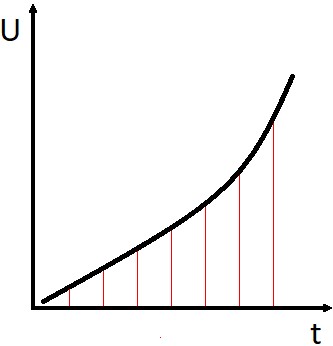
\includegraphics[width=8cm]{discretization}
    \centering
  \end{figure}

  Характеристика, отражающая эти временные промежутки, называется частота
  дискретизации.
\item \emph{Квантование.} Полученные значения заменяются ближайшим значением из
  набора фиксированных величин -- \emph{уровней квантования}
  (\ref{fig:quantization}.)

  \begin{figure}[h]
    \caption{Квантование.}
    \label{fig:quantization}
    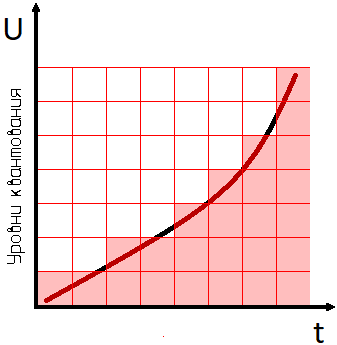
\includegraphics[width=8cm]{quantization}
    \centering
  \end{figure}

\item \emph{Кодирование.} Квантованным значениям присваивается цифровой код
  (\ref{fig:coding}.)

  \begin{figure}[h]
    \caption{Кодирование.}
    \label{fig:coding}
    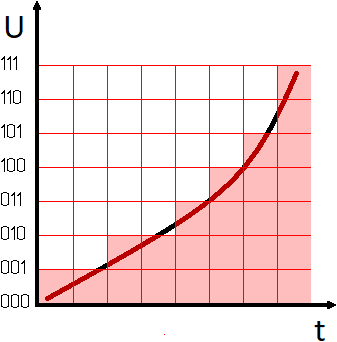
\includegraphics[width=8cm]{coding}
    \centering
  \end{figure}

  Чем выше частота дискретизации и чем больше уровней квантования, тем точнее
  преобразование.

\end{enumerate}

Одной из характеристик АЦП является \emph{разрядность}. Она определяет
количество значений, которое может выдать АЦП. Посмотрим на последний график:
для кодирования значений используется три бита, значит АЦП, описываемый таким
графиком, имеет, соответственно, разрядность 3 бита. То есть $ 2^3 = 8 $, что
равно количеству уровней квантования.

Вот и ответ на поставленный вопрос. АЦП Arduino 10-ти разрядный, $2^10 = 1024$.
Именно столько значений АЦП Arduino может выдать.

Ещё есть такое устройство как ЦАП - \emph{Цифро-Аналоговый Преобразователь},
который, как нетрудно догадаться, выполняет функцию, обратную функции АЦП -
преобразует цифровой сигнал в аналоговый. Область применения ЦАП и АЦП
достаточно широка: в звуковых и видео- картах, в мониторах, в различной
акустической аппаратуре, в измерительных приборах, и многих других видах
техники.

Стоит упомянуть про 8-битную музыку в древних игровых консолях. Её название
отражает разрядность ЦАП звуковых чипов тех консолей -- 8 бит. Именно такой ЦАП
позволял выдавать тот самый резковатый, хлопающий и шипящий звук.

%%%%%%%%%%%%%%%%%%%%%%%%%%%%%%%%%%%%%%%%%%%%%%%%%%%%%%%%%%%%%%%%%%%%%%%%%%%%%%%%
\chapter{Широтно-импульсная модуляция}

\section{Общее описание принципов работы}

Широтно-импульсная модуляция, или сокращённо \emph{ШИМ}, позволяет выдавать на
цифровом порту Arduino напряжение в диапазоне от 0 до 5 вольт, используя при
этом только два сигнала -- \texttt{HIGH} (логическая единица, при которой на
порт подается 5 В) и \texttt{LOW} (логический ноль, при котором на порт подается
0 В.) Меняя быстро данные значения на порту, можно добиться, например,
напряжения в 2.5 В.

\section{Длина волны}

При создании ``мигающего светодиода'' мы попеременно подавали на цифровой порт
сигналы \texttt{HIGH} и \texttt{LOW}, с указанием задержки (в миллисекундах).
Если мы посмотрим на вид сигнала на цифровом порту во времени (скажем, с помощью
осциллографа), то увидим примерно следующую картину:


Где \emph{длина периода} -- расстояние между двумя ближайшими друг к другу
точками в пространстве, в которых колебания происходят в одинаковой фазе.

Зная длину периода, можно рассчитать \emph{частоту колебаний}, и наоборот --
зная частоту, можно рассчитать длину волны.

При работе с ШИМ мы будем использовать длину периода, заданную в микросекундах
(мкс). 1 микросекунда -- это одна миллионная часть секунды. Для краткости записи
подобных маленьких величин часто используется возведение числа 10 в
отрицательную степень. Ниже приведена таблица с указанием различных долей
секунды\footnote{Для полного списка кратных и дольных единиц см. статью
\href{https://ru.wikipedia.org/wiki/\%D0\%A1\%D0\%B5\%D0\%BA\%D1\%83\%D0\%BD\%D0\%B4\%D0\%B0}{Секунда}
в Википедии.}:

\begin{tabular}{p{4cm}|p{4cm}|p{6cm}}
  Название & Величина & Пример \\
  \hline \hline
  секунда (с) & $ 1 с $ или $ 10^0 с $ & $ 500 * 10^{0} = 500 с $ \\
  \hline
  миллисекунда (мс) & $ 0.001 c $ или $ 10^{-3} c $ & $ 500 * 10^{-3} = 500 мс $ \\
  \hline
  микросекунда (мкс) & $ 0.000001 c $ или $ 10^{-6} c $ & $ 500 * 10^{-6} = 500 мкс $ \\
  \hline
  наносекунда (нс) & $ 0.000000001 c $ или $ 10^{-9} с $ & $ 500 * 10^{-9} = 500 нс $
\end{tabular}

\section{Коэффициент заполнения}

Каким образом задается напряжение из диапазона? Очень просто: путём изменения
времени подачи того или иного сигнала. Чем больше времени на порту сигнал HIGH,
тем выше напряжение. При этом, длина периода \texttt{P} остаётся фиксированной
(например, 1000 микросекунд). Таким образом для ШИМ важно процентное отношение
одного сигнала к другому, и, увеличивая время подачи одного сигнала, следует
уменьшать время подачи другого (следовательно если мы подаем сигнал
\texttt{HIGH} 60\% от отведенного времени, нужно заполнить оставшиеся 40\%
сигналом \texttt{LOW}).

Отношение периода следования сигнала к длительности импульса называется
\emph{скважностью}. В англоязычной литературе величина, обратная скважности,
называется \emph{коэффициентом заполнения} (англ. \emph{duty cycle}).

Мы будем использовать термин ``коэффициент заполнения''.

\example {
  Мы хотим получить 2.5 вольта на цифровом порту 2, имея в
  распоряжении только два значения -- 0 В и 5 В. Для этого нам потребуется
  реализовать ШИМ с коэффициентом заполнения 50\%. При длине волны в 1000
  микросекунд мы должны половину времени (500 микросекунд) заполнить
  положительным сигналом (сигнал \texttt{HIGH}) и подать его на выбранный порт, затем
  остальную часть заполним отрицательным сигналом (сигналом \texttt{LOW}).
  Если всё сделано правильно, то на 2 цифровом порту получим 2.5 вольта.
}

Для генерации нужного сигнала нам потребуется создать инструмент
(\emph{функцию}), который впоследствии мы будем использовать. Мы уже говорили о
важности написания и использования собственных функций в программе -- функции
позволяют нам создавать модульные программы, упрощают поддержку существующего
программного кода и написание нового кода.

Подумаем над тем, какой должна быть наша функция, реализующая ШИМ. Ниже приведён
знакомый нам график, отображающий сигнал на цифровом порту -- мы будем
использовать этот график, как основу для написания функции.

%% TODO: Add the graph.

В программе мы обозначим длину периода константой \texttt{P}, равной 1000 мкс.
Значения задержек, заданных переменными \texttt{d1} и \texttt{d2}, необходимо
вычислить на основе коэффициента заполнения, задаваемого параметром функции
\texttt{duty\_cycle} (который задаётся дробным значением -- к примеру, 0.5.)

Имея перед глазами этот график, нетрудно набросать словесное описание функции
(назовём функцию \texttt{pwm}, как сокращение от англ. \emph{pulse width
  modulation}.)

Начнём с того, что, скорее всего, подобная функция должна принимать три
параметра:
\begin{enumerate}
\item Номер порта (обозначаемый целым числом), на котором следует сгенерировать
  ШИМ сигнал; назовём этот параметр \texttt{pin}.
\item Коэффициент заполнения, заданный дробным числом -- к примеру, 50\% будет
  задано, как 0.5; назовём этот параметр \texttt{duty\_cycle}
\item Длина ШИМ сигнала в микросекундах; назовём этот параметр
  \texttt{signal\_length}.
\end{enumerate}

Запишем тоже самое на языке С++:

\begin{verbatim}
void pwm(int pin, float dc, long signal_length) {
  // тело функции
}
\end{verbatim}

О том, что такое \texttt{void}, будет сказано позже, пока что стоит принять как
факт, что это начало объявления функции. Наверняка появились вопросы по новым
типам переменных -- \texttt{float} и \texttt{long}. Почему нельзя использовать
привычный \texttt{int}? Дело в том, что переменная типа \texttt{int} не может
хранить дробные числа, а также имеет диапазон значений от -32 768 до 32 767. Для
хранения дробных чисел используется \texttt{float}, а для чисел, не входящих в
диапазон \texttt{int}, стоит использовать \texttt{long}, имеющий диапазон от -2
147 483 648 до 2 147 483 647. Теперь подумаем над телом функции. Первым делом
нам необходимо задать константу \texttt{P}:

\begin{verbatim}
const int P = 1000; // мкс
\end{verbatim}

Обратите внимание, что мы используем ключевое слово const для того, чтобы
пометить \texttt{WAVE\_LENGTH}, как константу -- мы всё равно не собираемся
менять это значение. Кроме того, мы указали в комментарии, что значение задано в
микросекундах (мкс), что упрощает чтение кода. В C++, да и в других языках,
константа -- это та же переменная, но её значение нельзя менять после её
объявления.

Следующим этапом будет вычисление в теле функции значений переменных \texttt{d1}
и \texttt{d2} на основе значения \texttt{duty\_cycle}, заданного при вызове
функции:

\begin{verbatim}
int d1 = P * duty_cycle;
int d2 = P - d1;
\end{verbatim}

Видно, что как только мы вычислили \texttt{d1}, вычислить \texttt{d2} не
составляет труда. Осталось только посчитать, сколько раз нужно повторить волну
длиной \texttt{P}, чтобы сгенерировать сигнал длиной \texttt{signal\_length}:

\begin{verbatim}
int count = signal_length / P;
\end{verbatim}

Теперь у нас есть всё, что нужно для генерации нужного нам сигнала. Поскольку
исходя из описания выше нам нужно будет повторять волну count раз, то для этого
удобно использовать цикл \texttt{for} (цикл со счётчиком):

\begin{verbatim}
for (int c = 0; c < count; c++) {
  digitalWrite(pin, HIGH);
  delayMicroseconds(d1);
  digitalWrite(pin, LOW);
  delayMicroseconds(d2);
}
\end{verbatim}

Готово! Осталось только задействовать функцию pwm в нашей программе.

\subsection{Задачи}

\begin{enumerate}
\item Написать программу, плавно включающую и выключающую светодиод. Собрать и
  протестировать схему. 
\item Написать программу, реализующую ``бегущий огонь'' с использованием ШИМ.
  Собрать и протестировать схему.
\item Используя потенциометр, модифицировать систему из задания №2 таким
  образом, чтобы можно было регулировать яркость ``бегущего огня''.
\item Разработать ``бегущий огонь'', где следующий светодиод начинает плавно
  разгораться одновременно с затуханием предыдущего светодиода.
\end{enumerate}

%% \section{Последовательный порт}

%% \subsection{Сбор и обработка данных на стороне компьютера}

%% Другой задачей, решаемой с помощью функций записи данных в последовательный
%% порт, является сбор данных на стороне компьютера. Arduino IDE позволяет нам
%% визуализировать данные через специальный плоттер (доступ к которому можно
%% получить, выбрав в меню ``Инструменты'' пункт ``Плоттер по последовательному
%% соединению'', либо нажав комбинацию клавиш \hotkey{Ctrl + Shift + L}.)

%% \subsection{Передача данных с компьютера на Arduino}

%% Передавать данные с Arduino на компьютер мы уже научились. Теперь посмотрим на
%% передачу данных в обратном направлении. Для того чтобы передать данные с
%% компьютера на Arduino также необходимо выполнить настройку последовательного
%% порта; кроме этого, нам потребуется задействовать несколько новых функций.

%% \subsubsection{Чтение отдельных байт}

%% Функция \texttt{Serial.read} читает байт данных из поступивших на Arduino. То
%% есть возвращает вам некое целое число, с которым вы вольны делать что вашей душе
%% угодно. Каждый вызов этого метода будет возвращать вам следующий байт данных из
%% тех что поступили на Arduino. Если возвращать нечего, то есть вы считали все что
%% было, данная функция вернет -1.

%% \note{ Если передаются именно байты, возникает проблема: -1 это 0xFF в
%%   шестнадцатиричной системе, или 255 в десятичной. Такой же байт, как и все
%%   остальные, из-за чего невозможно. поэтому нужно сперва вызывать функцию available . }

%% Допустим мы отправили 1 байт данных на Arduino и использовали нижеприведенный
%% участок кода:

%% \begin{verbatim}
%% int incoming_byte;
%% void loop() {
%%   if (Serial.available() > 0) {
%%       incoming_byte = Serial.read();
%%   }
%% }
%% \end{verbatim}

%% После того, как вы считаете байт данных, он будет перемещен в вашу переменную
%% \texttt{incoming\_byte} а функция \texttt{Serial.available} снова будет
%% возвращать 0, пока не поступят новые данные.

%% То есть, когда вы считываете байт, показания счетчика принятых байт уменьшается
%% и \texttt{Serial.available} будет показывать на 1 байт меньше.

%% Помните, что функция \texttt{Serial.read} возвращает только 1 байт данных, если
%% например вы передали 4 символа каждый по 1 байту, вам потребуется 4 раза вызвать
%% данную функцию чтобы прочитать эти символы и самостоятельно позаботится о том
%% чтобы разместить их в массив символов либо воспользоваться функцией
%% \texttt{Serial.readBytes}.

%% \subsubsection{Чтение чисел}

%% Функция \texttt{Serial.parseInt} просматривает данные, поступившие на Arduino, и
%% ищет среди них набор кодов (чисел) от 48 до 57, которые соответствуют символам
%% чисел от 0 до 9 и преобразует все это в правильное целочисленное значение. Таким
%% образом если вы с монитора порта передадите "число" (на самом деле, строку)
%% ``72'', данный метод увидит 2 последовательных байта 55 и 51, корректно
%% преобразует его в число 72 и вернет его как правильное целочисленное значение.
%% Давайте напишем маленькую эхо-программу, которая покажет принцип работы данной
%% функции и позволит вам узнать какому символу соответствует то или иное число.

%% \begin{verbatim}
%% int incoming_int = 0;

%% void setup()
%% {
%%   Serial.begin(9600);
%%   Serial.setTimeout(2000);
%% }
%% void loop()
%% {
%%   if (Serial.available() > 0)
%%   {
%%     incoming_int = Serial.parseInt();
%%     Serial.write(incoming_int);
%%   }
%% }
%% \end{verbatim}

%% Данная программа будет работать так. Если в мониторе порта вы введете строку
%% ``72'' то монитор порта отправит его на Arduino как два байта данных в виде
%% чисел 55 и 51, функция \texttt{Serial.parseInt} подождет 2000 миллисекунд (как
%% видите я поменял время ожидание с 1 секунды на 2 секунды, чтобы нагляднее
%% показать кое какие аспекты) увидит эти два значения и преобразует их в одно
%% целочисленное 72 и присвоит его переменной \texttt{incoming\_int}, мы с помощью
%% метода \texttt{Serial.write} передадим число 72 как есть обратно в монитор порта
%% (почему именно этот метод нужен читайте далее) где монитор порта корректно
%% преобразует число 72 в соответствующий символ и покажет нам символ ``H'' который
%% соответствует коду 72. Таким образом мы можем передавать числовые значения с
%% компьютера на платформу Arduino и дальше использовать эти значения.

\chapter{Синтез музыки и технологии}

\section{Звук}

Как известно \emph{звук} -- это колебания (вид сигнала), и каждому определённому
звуку соответствует своя частота колебаний.

Частоты измеряются в \emph{Герцах} (Гц), и один Герц (1 Гц) означает одно
колебание в секунду. 10 колебаний в секунду -- 10 Гц, 100 колебаний в секунду --
100 Гц и т. д. Если же мы говорим про частоты в 100 Гц и более, то удобнее
использовать приставки Кило- (КГц), Мега- (МГц) и Гига- (ГГц): сигнал с частотой
1 КГц поданный на цифровой порт колеблет мембрану динамика 1000 раз в секунду.
Ниже приведена таблица некоторых кратных единиц частот в Герцах:

\begin{tabular}{p{3cm}|p{4cm}|p{3.5cm}}
  Название & Величина & Пример \\
  \hline \hline
  Герц (Гц)
  & $ 1 \mbox{Гц} $ или $ 10^0 \mbox{Гц} $
  & $ 100 * 10^0 \mbox{Гц} = 100 \mbox{Гц} $ \\
  \hline
  Килогерц (КГц)
  & $ 1000 \mbox{Гц} $ или $ 10^3 \mbox{Гц} $
  & $ 100 * 10^3 \mbox{Гц} = 1 \mbox{КГц} $ \\
  \hline
  Мегагерц (МГц)
  & $ 1000000 \mbox{Гц} $ или $ 10^6 \mbox{Гц} $
  & $ 100 * 10^6 \mbox{Гц} = 1 \mbox{МГц} $ \\
  \hline
  Гигагерц (ГГц)
  & $ 1000000000 \mbox{Гц} $ или $ 10^9 \mbox{Гц} $
  & $ 100 * 10^9 \mbox{Гц} = 1 \mbox{ГГц} $ \\
\end{tabular}

Таким образом, для генерации сигнала нам необходимо знать его частоту в Герцах,
либо знать длину волны.

Зная период, мы можем узнать частоту, и наоборот -- поскольку частота является
ничем иным, как количеством повторений заданных колебаний в секунду. Это удобно
представить визуально (\ref{fig:sound-fig-1}.)

\begin{figure}[h]
  \caption{Визуальное представление частоты колебаний 5 Гц.}
  \label{fig:sound-fig-1}
  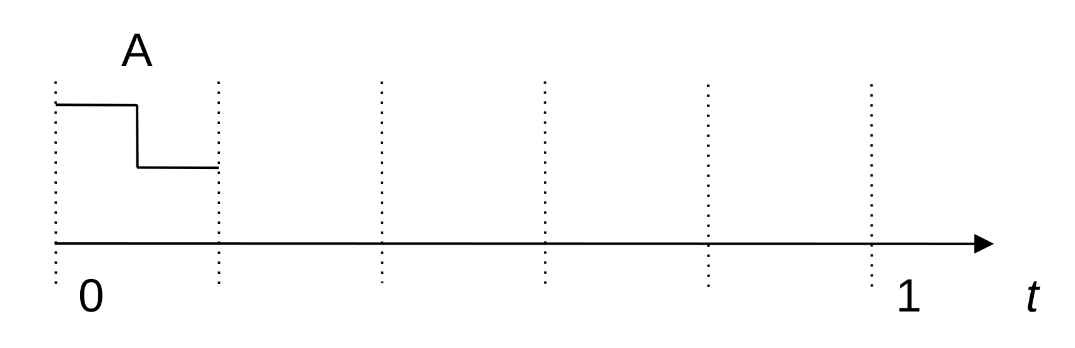
\includegraphics[width=10cm]{sound-fig-1}
  \centering
\end{figure}

Если известно, что колебание А помещается 5 раз в 1 секунду, то говорят, что
частота данного сигнала равна 5 Гц. Узнать период можно, разделив 1 секунду
(заданную в микросекундах) на частоту (5 Гц):

\begin{equation}
  \frac{1000000 \mbox{мкс}}{5 \mbox{Гц}} = 200000 \mbox{мкс}
\end{equation}

Получается, что длина волны равна 200000 мкс, или $ 200 * 10^3 \mbox{мс} $. Если
же нам известна длина волны и нужно узнать частоту, то необходимо разделить 1
секунду (в микросекундах) на длину волны -- таким образом, получим частоту в
Герцах. Всё просто.

Метод генерации звука похож на ШИМ. Основные отличия заключаются в том, что
теперь мы должны изменять длину волны len, оставляя коэффициент заполнения
неизменным -- он описывается константой DC и всегда равен 0.5. Поскольку
коэффициент заполнения всегда равен 50\% (0.5), то время подачи сигналов
\texttt{HIGH} и \texttt{LOW} всегда одинаково -- иными словами, нам достаточно
вычислить только задержку \texttt{d1}. Это показано на графике ниже:

Как и в случае с ШИМ, начнём писать функцию, которая будет реализовывать
вышеописанные принципы. Функция будет называться \texttt{play\_tone} и будет
позволять генерировать звук с нужной частотой на указанном цифровом порту.

Посмотрим, что данная функция должна принимать в качестве параметров:
\begin{enumerate}
\item Номер цифрового порта, к которому подключен динамик и куда будет
  выводиться звук; назовём этот параметр ``pin'';
\item Частота ``f'', измеряемая в Герцах. 
\item Длина звукового сигнала; назовём этот параметр ``t''.
\end{enumerate}

На языке C++ это будет выглядеть примерно так:
\begin{verbatim}
void play_tone(int pin, float f, long t) {
    // тело функции
}
\end{verbatim}

Теперь пришло время написать тело функции. Начнём с того, что зададим
коэффициент заполнения в виде константы:
\begin{verbatim}
const float DC = 0.5; // 50%
\end{verbatim}

Теперь из частоты найдём период \texttt{p}:
\begin{verbatim}
long p = 1000000 / f;
\end{verbatim}

Далее посчитаем длину задержки \texttt{d}:
\begin{verbatim}
int d = p * DC;
\end{verbatim}

И посчитаем, сколько раз нам нужно повторить период длиной p микросекунд, чтобы
заполнить время \texttt{t}:
\begin{verbatim}
int count = t / p;
\end{verbatim}

Почти всё готово. Осталось только написать цикл, который будет генерировать
заданную волну нужное количество раз. Здесь отлично подойдёт цикл со счётчиком
(\texttt{for}):

\begin{verbatim}
for (int c = 0; c < count; c++) {
  digitalWrite(pin, HIGH);
  delayMicroseconds(d);
  digitalWrite(pin, LOW);
  delayMicroseconds(d);
}
\end{verbatim}

В общем виде, функция выглядит так:

\begin{verbatim}
void play_tone(int port, float f, long t) {
  const int T = 1000000 / f;
  int d = T / 2;
  int count = t / T;
  for (int i = 0; i < count; i++) {
    digitalWrite(port, HIGH);
    delayMicroseconds(d);
    digitalWrite(port, LOW);
    delayMicroseconds(d);
  }
}
\end{verbatim}

Наша функция генерации звука завершена. Теперь нам нужно подключить динамик к
Arduino и протестировать нашу систему.

\note{Во многих случаях одна и та же задача может быть решена несколькими
  способами. К примеру, функция \texttt{play\_tone} может быть реализована
  иначе; предложенная нами реализация является только одной из корректных. Как
  вариант, вы можете реализовать вариант функции, которая оперирует не длиной
  волны, а частотой. Подумайте над этим в свободное время. И не бойтесь
  экспериментировать! }

%%%%%%%%%%%%%%%%%%%%%%%%%%%%%%%%%%%%%%%%%%%%%%%%%%%%%%%%%%%%%%%%%%%%%%%%%%%%%%%%
\section{Подключение динамика}

Есть несколько вариантов динамиков, которые вы можете встретить. Например, есть
обычные динамики, где мембрана колеблется магнитным полем и тем самым создаёт
колебания воздуха, которые мы слышим, как звук. Есть пьезодинамики, в которых
звук генерируется за счёт обратного пьезоэлектрического эффекта -- механической
деформации пьезоэлектрика под действием электрического поля.\footnote{См. статью
"Пьезоэлектрический эффект" в Википедии для более подробного описания эффекта.}

Подключение и обычных динамиков и пьезодинамиков похоже; для наших задач
подойдёт как пьезодинамик ``для Arduino'', так и обычный динамик-пищалка из
персонального компьютера (а вы знали, что у вас в компьютере к системной плате
подключен динамик?)

Схема подключения представлена на рис. \ref{fig:sound-fig-2}.

%% TODO: Перерисовать схему.  Убрать резистор.
\begin{figure}[h]
  \caption{Подключение динамика-''пищалки'' к Arduino Mega 2560.}
  \label{fig:sound-fig-2}
  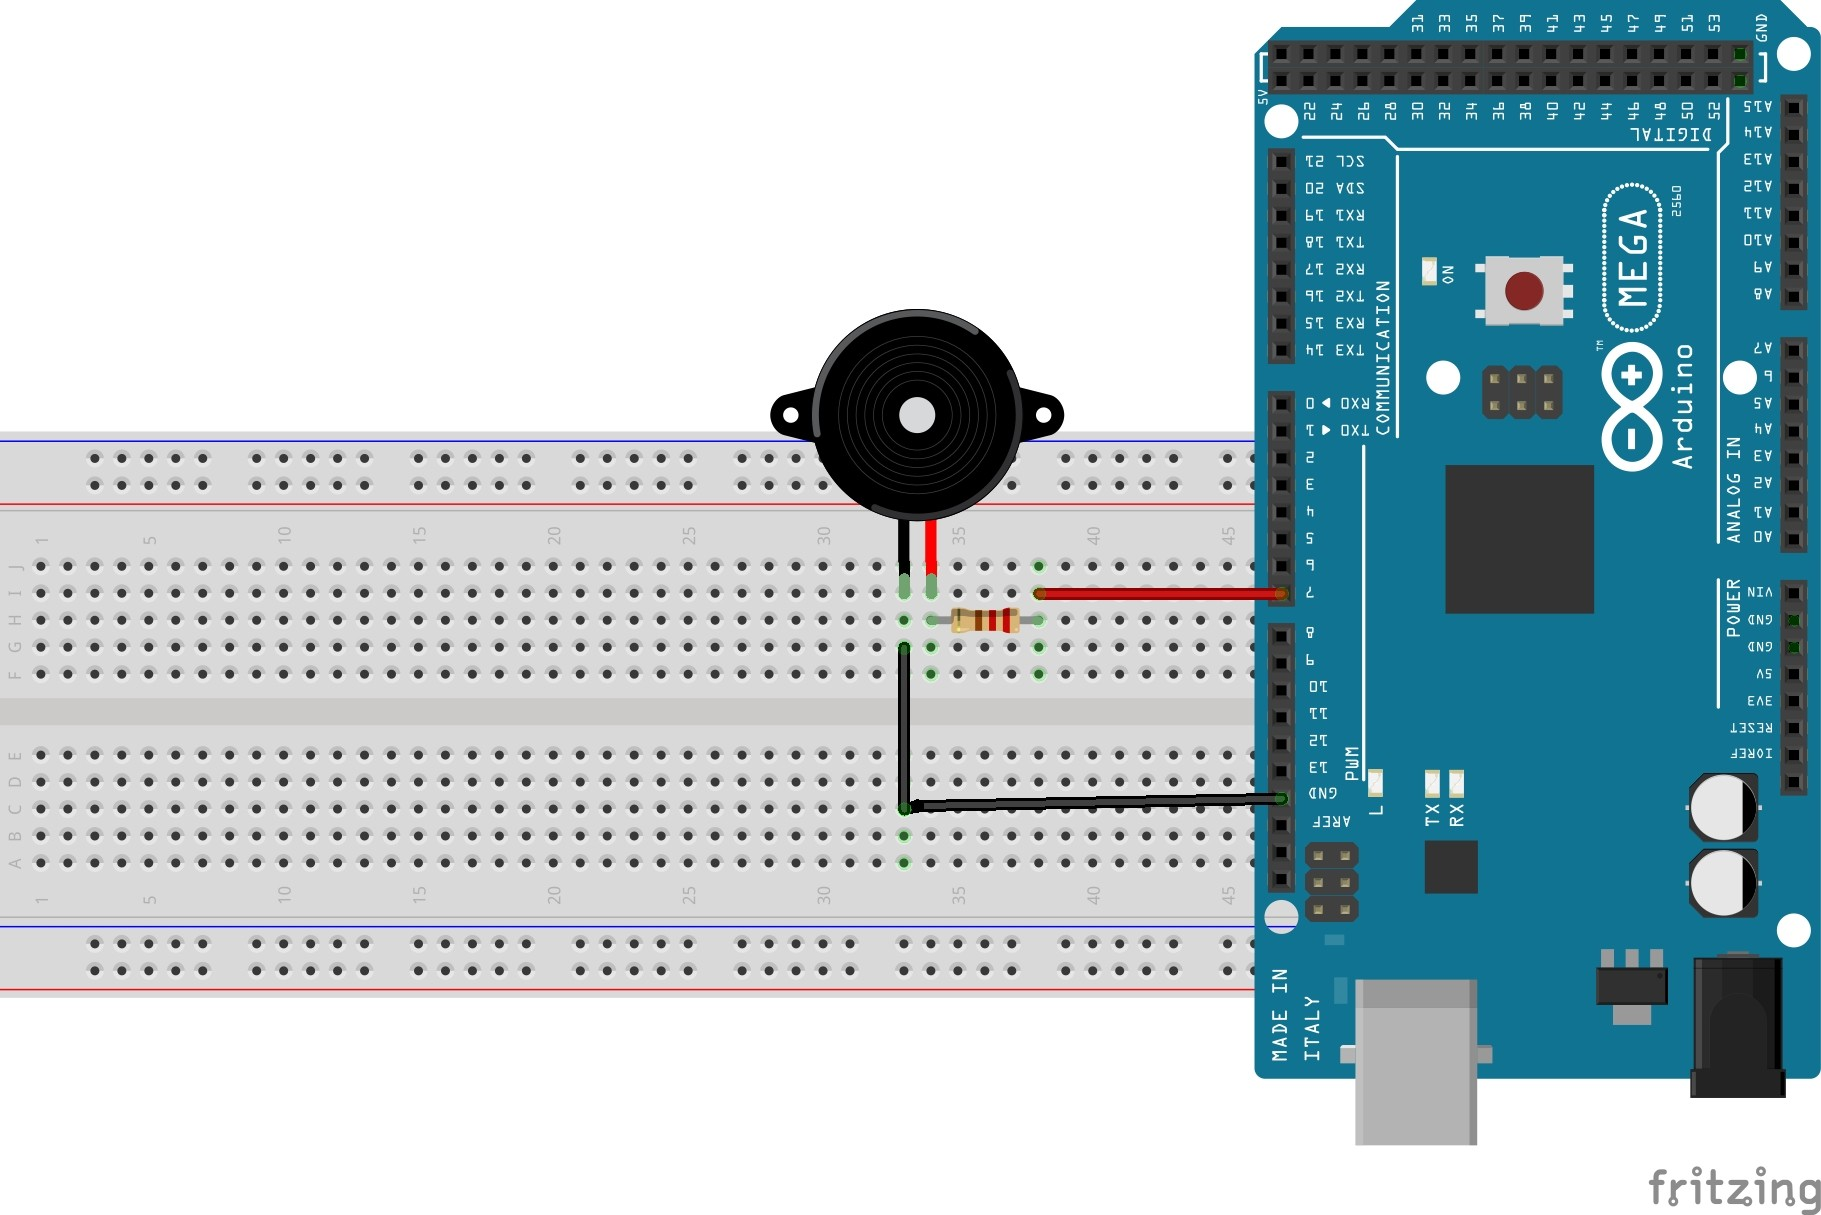
\includegraphics[width=10cm]{sound-fig-2}
  \centering
\end{figure}

Соберём указанную схему на макетной плате, и загрузим нашу программу генерации
звука в Arduino. Не забудьте добавить в тело функции loop вызов нашей функции
\texttt{play\_tone} и настроить цифровой порт, к которому подключен динамик, на
вывод.

Порт, к которому подключен динамик, лучше задать в виде константы
\texttt{SPEAKER\_PIN} в самом начале программы (до функции \texttt{setup}.)

\subsection{Задачи}
\begin{enumerate}
\item Сгенерируйте постоянный сигнал с частотой 261.63 Гц.
\item Сделайте так, чтобы сигнал менялся между 261.63 Гц и 349.23 Гц с частотой
  в 1 секунду. 
\item Модифицируйте систему таким образом, чтобы частота сигнала зависела от
  положения ручки потенциометра. 
\item Сделайте включение звукового сигнала по нажатию кнопки.
\end{enumerate}

Теперь мы можем генерировать звуковой сигнал с нужной нам частотой. Однако, если
мы хотим сгенерировать что-нибудь интересное -- вроде мелодии -- то нам
потребуется использовать вполне определённые частоты. Здесь нам очень кстати
будет хотя бы начальное знание музыкальной теории, но если таких знаний нет --
не беда, разберём по ходу дела.

%%%%%%%%%%%%%%%%%%%%%%%%%%%%%%%%%%%%%%%%%%%%%%%%%%%%%%%%%%%%%%%%%%%%%%%%%%%%%%%%
\section{Теория ритма}

Наш путь в музыку начнётся с разбора теории построения \emph{ритмов}. Думаю,
большинство из нас представляют, что такое ритм -- у многих именно он вызывает
например рефлекс покачивания головой в такт, или машинальное отстукивание ритма
на столешница стола, когда думаем над чем-то.

Чтобы понять, как строится ритм, необходимо знать две простые вещи, о которых мы
сейчас поговорим.

%%%%%%%%%%%%%%%%%%%%%%%%%%%%%%%%%%%%%%%%%%%%%%%%%%%%%%%%%%%%%%%%%%%%%%%%%%%%%%%%
\subsection{Понятие \emph{такта}}

Во-первых, музыкальное произведение делится на отрезки времени, называемые
\emph{тактами} -- как правило одинаковой длительности.\footnote{Музыка отличается
большим разнообразием, и композиторы придумывают всё новые трюки, как получить
желаемое впечатление у слушателя, поэтому здесь мы говорим с некоторыми
допущениями.}

На рисунке ниже показано, как может выглядеть музыкальная композиция из шести
тактов:

\begin{tikzpicture}
  \draw[thick, ->] (0, 0.5) -- (12, 0.5) node[anchor=north west] {t};
  \foreach \x/\n in {0/1, 2/2, 4/3, 6/4, 8/5, 10/6} {
    \draw (\x, 0) -- (\x, 1) -- (\x, 1) node[midway, above] {\n};
  };
\end{tikzpicture}

Протяжённость одного такта во времени определяется быстротой ритма, и про это мы
поговорим позже. Пока можно представить, что один отрезок занимает одну условную
единицу времени. Можете принять эту условую единицу за отрезок времени, удобный
для вашего восприятия -- например, одну секунду.

Во-вторых, эти такты делятся на ещё на более мелкие части, по которым, как по
``ячейкам'', раскладываются различные звуки. Достаточно большая часть музыки
пронизана математикой, и первое математическое, с чем мы столкнёмся -- это
простые дроби. Одним из популярных способов деления такта на части является
$\frac{4}{4}$ или, по-другому называемый ``четыре четверти''. В таком способе
деления такта в него умещается ровно единица некоторого условного времени, про
которое мы говорили выше.\footnote{Существуют более сложные способы деления
такта на части, которые дают суммарное значение меньше или больше единицы -- про
это мы поговорим позднее.}

Если мы поделим каждый такт на четыре части, то получим следующую картину:

\begin{tikzpicture}
  \draw[thick, ->] (0, 0.5) -- (12, 0.5) node[anchor=north west] {t};
  \foreach \x/\n in {0/1, 2/2, 4/3, 6/4, 8/5, 10/6} {
    \draw (\x, 0) -- (\x, 1) -- (\x, 1) node[midway, above] {\n};
  };

  \foreach \x/\n in {0, 0.5, ..., 10} {
    \draw (\x, 0) -- (\x, 0.5);
  };
\end{tikzpicture}

Возьмём отдельный такт и посмотрим на него внимательно:

\begin{tikzpicture}
  \draw[thick] (0, 0.5) -- (8, 0.5) node[anchor=north west] {t};
  \foreach \x/\n in {0/1, 8/2} {
    \draw (\x, 0) -- (\x, 1)  -- (\x, 1) node[midway, above] {\n};
  };

  \foreach \x in {0, 2, ..., 6} {
    \draw (\x, 0) -- (\x, 0.5) node[pos=0.25, right] {$ \frac{1}{4} $};
  };
\end{tikzpicture}

Если просуммируем все части, то снова получим единицу:

\begin{equation}
  \frac{1}{4} + \frac{1}{4} + \frac{1}{4} + \frac{1}{4} = \frac{1}{1}
\end{equation}

На каждую из четвертей можно задать какой-то звук -- пока нам не важно, насколько
он будет музыкальный. Допустим, что три четверти будут звучать с частотой 50Гц,
и одна часть -- с частотой 100Гц:

\begin{tikzpicture}
  \draw[thick] (0, 0.5) -- (8, 0.5) node[anchor=north west] {t};
  \foreach \x/\n in {0/1, 8/2} {
    \draw (\x, 0) -- (\x, 1) -- (\x, 1) node[midway, above] {\n};
  };

  \foreach \x in {0, 2, ..., 6} {
    \draw (\x, 0) -- (\x, 0.5) node[pos=0.25, right] {$ \frac{1}{4} $};
  };

  \foreach \x/\freq in {0/50, 2/50, 4/50, 6/100} {
    \draw (\x, 0) -- (\x, 0.5) node[pos=1.5, right] {\freq Гц};
  };
\end{tikzpicture}

Поздравляю -- мы только что получили с простой ритм. Попробуем запрограммировать
его, беря за длину такта \texttt{T} одну секунду, или 1000000 (миллион)
микросекунд.

Между ``ударами'' необходимо поставить короткую задержку (например, в 100 мс),
чтобы удары одинаковой частоты, идущие один за другим, не сливались в один
долгий звук.

\begin{verbatim}
// Номер порта, куда подключен динамик.
const int SPEAKER = 2;

void setup() {
  pinMode(SPEAKER, OUTPUT);
}

// Функция воспроизведения звука указанной частоты.
void play_tone(int port, float f, long t) {
  const int T = 1000000 / f;
  int d = T / 2;
  int count = t / T;
  for (int i = 0; i < count; i++) {
    digitalWrite(port, HIGH);
    delayMicroseconds(d);
    digitalWrite(port, LOW);
    delayMicroseconds(d);
  }
}

void loop() {
  const long T = 1000000; // Длина такта в микросекундах
  play_tone(SPEAKER, 50, T / 4); // Четверть
  delay(100); // Задержка между звуками
  play_tone(SPEAKER, 50, T / 4); // Четверть
  delay(100);
  play_tone(SPEAKER, 50, T / 4); // Четверть
  delay(100);
  play_tone(SPEAKER, 100, T / 2); // Половина
  delay(100);
}
\end{verbatim}

Можно теперь взять что-то посложнее.

\subsection{Более сложные ритмы}

Возможно некотыре из вас знают такую зажигательную композицию, как ``We Will
Rock You'' в исполнении группы Queen\footnote{Официальное музыкальное видео на
данную композицию можно посмотреть здесь:
\url{https://www.youtube.com/watch?v=-tJYN-eG1zk}}. Данная композиция имеет
чётко выраженный, легко узнаваемый ритм, который можно упрощенно описать как
``два притопа, один прихлоп'', вокруг которого строится вся композиция -- вы сами
можете достаточно легко повторить этот ритм, коротко топая ногой два раза, и
потом делая ``долгий'' хлопок руками.

Структура этого ритма может быть описана следующим набором простых дробей
(\ref{fig:queen-we-will-rock-you-rhythm-1}.) Частоты звуков мы опять же берём
произвольно.

\begin{figure}[ht]
  \label{fig:queen-we-will-rock-you-rhythm-1}
  \caption{Ритм мелодии ``We Will Rock You''}
  \begin{tikzpicture}
    \draw[thick] (0, 0.5) -- (8, 0.5) node[anchor=north west] {t};
    \foreach \x/\n in {0/1, 8/2} {
      \draw (\x, 0) -- (\x, 1) -- (\x, 1) node[midway, above] {\n};
    };

    \foreach \x in {0, 2} {
      \draw (\x, 0) -- (\x, 0.5) node[pos=0.25, right] {$ \frac{1}{4} $};
    };

    \draw (4, 0) -- (4, 0.5) node[pos=0.25, right] {$ \frac{1}{2} $};

    \foreach \x/\freq in {0/50, 2/50} {
      \draw (\x, 0) -- (\x, 0.5) node[pos=1.5, right] {\freq Гц};
    };
    \draw (4, 0) -- (4, 0.5) node[pos=1.5, right] {100 Гц};
  \end{tikzpicture}
\end{figure}

Как мы видимо из рисунка \ref{fig:queen-we-will-rock-you-rhythm-1}, деление
такта на части не обязательно должно быть всегда равномерным -- здесь мы получили
две четверти, и одну половину. Суммарно же у нас опять выходит единица (см.
формулу \ref{equation:queen-we-will-rock-you-rhythm-1}.) Попутно вспоминаем, что
для сложения простых дробей нам необходимо их привести к общему знаменателю.

\begin{equation}
  \label{equation:queen-we-will-rock-you-rhythm-1}
  \frac{1}{4} + \frac{1}{4} + \frac{1}{2} = \frac{1}{4} + \frac{1}{4} + \frac{2}{4} = \frac{4}{4} = \frac{1}{1} = 1
\end{equation}

%%%%%%%%%%%%%%%%%%%%%%%%%%%%%%%%%%%%%%%%%%%%%%%%%%%%%%%%%%%%%%%%%%%%%%%%%%%%%%%%
\subsection{Музыкальная запись ритма}

С точки зрения музыкальной нотации, данный ритм можно записать примерно
следующим образом (см. рисунок \ref{fig:lilypond-queen-1}.)

\begin{figure}[ht]
  \caption{Ритм мелодии ``We Will Rock You'' в музыкальной нотации (упрощенная версия.)}
  \centering
  \begin{lilypond}
    \relative c' {
      \numericTimeSignature
      \time 4/4
      e,4 e4 e'2
    }
  \end{lilypond}
  \label{fig:lilypond-queen-1}
\end{figure}

Если вы не знакомы с музыкальной нотацией (т.е. способом записи музыки), и
изображение выглядит для вас совершенно непонятно, то не отчаивайтесь -- на
данном этапе нам достаточно увидеть, что есть три ``закорючки'', которые
обозначают звуки разной длительности: ``\quarterNote'' ($\frac{1}{4}$),
``\quarterNote'' ($\frac{1}{4}$) и ``\halfNote'' ($\frac{1}{2}$).

Расположение ``закорючек'' слева направо говорит нам о порядке ``извлечения''
звуков из музыкальных инстнументов, а каждый вид начертания ``закорючки''
соответствует длительности звука, согласно следующей таблице
(\ref{table:music-notes-legths}.)

\begin{table}[ht]
  \caption{Некоторые возможные длительности нот.}
\begin{tabular}{p{3cm}|p{4cm}|p{3.5cm}}
  Начертание & Длительность & Название \\
  \hline \hline
  \wholeNote     & $\frac{1}{1}$ & ``Целая'' \\
  \hline
  \halfNote      & $\frac{1}{2}$ & ``Половина'' \\
  \hline
  \quarterNote   & $\frac{1}{4}$ & ``Четверть'' \\
  \hline
  \eighthNote     & $\frac{1}{8}$ & ``Восьмая'' \\
  \hline
  \sixteenthNote & $\frac{1}{16}$ & ``Шестнадцатая'' \\
  \hline
\end{tabular}
\label{table:music-notes-legths}
\end{table}

Существуют и более длинные и более короткие ноты, но они встречаются реже, чем
перечисленные в таблице \ref{table:music-notes-legths}, поэтому для краткости мы
их рассматривать не будем.

Какие выводы мы можем сделать в итоге? Что в музыкальной нотации звуки, которые
необходимо ``извлечь'' из музыкального инструмента, записываются слева на право,
как и обычный, привычный нам русский текст (или английский, к слову говоря.)

Мы можем расположить музыкальную запись для удобства нашего понимания на
графике, где ось $\mbox{X}$, будет обозначать время, идущее слева направо:

\begin{figure}[ht]
  \caption{Музыкальный ``график''.}
  \centering
  \begin{lilypond}
    \relative c' {
      \numericTimeSignature
      \time 4/4
      e,4 e4 e'2
    }
  \end{lilypond}
  \begin{tikzpicture}
    \draw[thick, ->] (0, 0.5) -- (12, 0.5) node[anchor=north east] {Время};
  \end{tikzpicture}

  \label{fig:lilypond-queen-1}
\end{figure}

С точки зрения программирования, код воспроизведения ритма может быть следующим:

\begin{verbatim}
// Здесь пропущен уже известный вам код настройки системы и реализации
// функции воспроизведения звука.

void loop() {
  const long T = 1000000; // Длина такта в микросекундах
  play_tone(SPEAKER, 50, T / 4); // Четверть
  delay(100);
  play_tone(SPEAKER, 50, T / 4); // Четверть
  delay(100);
  play_tone(SPEAKER, 100, T / 2); // Половина
  delay(100);
}
\end{verbatim}

Теперь нам нужно более точно определить, какова длительность целого отрезка
времени, чтобы посчитать длину его частей.

%%%%%%%%%%%%%%%%%%%%%%%%%%%%%%%%%%%%%%%%%%%%%%%%%%%%%%%%%%%%%%%%%%%%%%%%%%%%%%%%
\subsection{Темп музыки}

\emph{Темпом} в музыке скорость исполнения музыки, если говорить упрощенно. В
современной музыке темп измеряется в \emph{ударах в минуту} (буквальный перевод
английского ``Beats per Minute'', сокращённо называемый \emph{BPM}.)

Темп в музыке может задаваться с помощью специального маятника, который
раскачивается из стороны в сторону с равномерной скоростью, делая удары (или
щелчки) в крайних положениях. Такой маятник называется \emph{метрономом}.

\begin{figure}[h]
  \caption{Схематическое изображение механического метронома (источник:
    \url{https://commons.wikimedia.org/wiki/File:Metronome_(PSF).png}).}
  \label{fig:sound-metronome}
  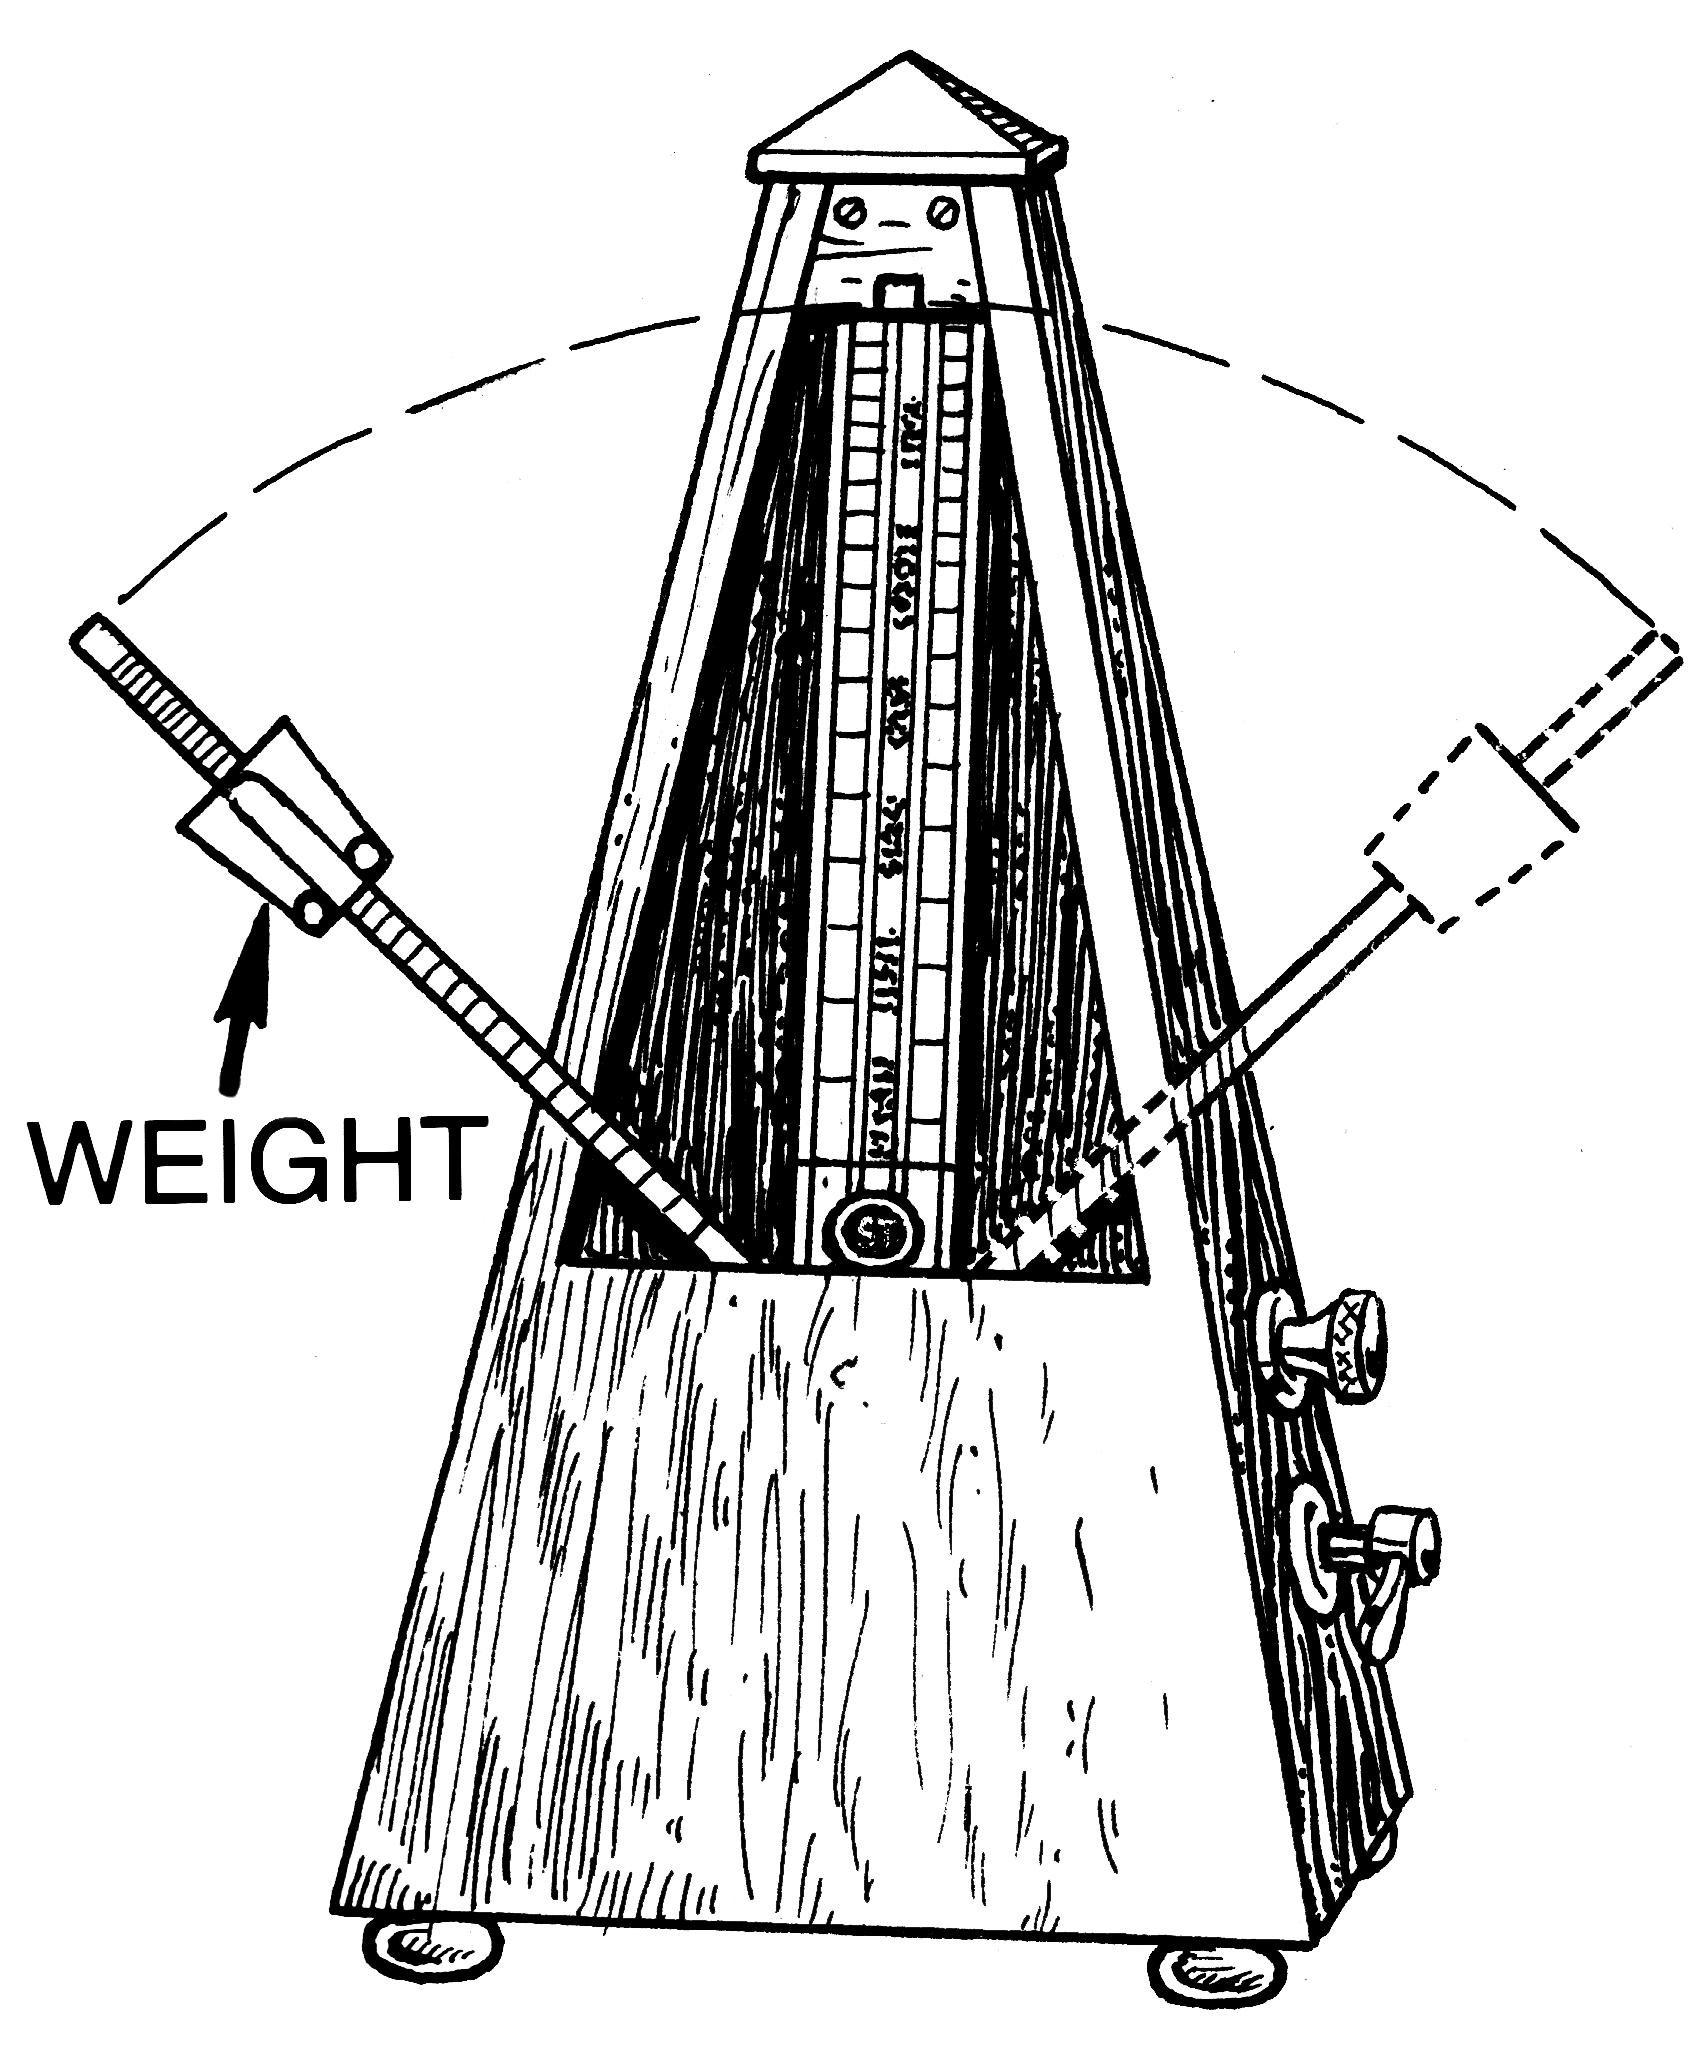
\includegraphics[width=10cm]{Metronome}
  \centering
\end{figure}

В современном мире роль механического маятника часто заменяет специальное
компактное электронное устройство или даже приложение для мобельного телефона,
издающее щелчки через равные промежутки времени с заданной скоростью.

Чем больше ударов в минуту, тем выше темп -- и выше скорость ритма. Примерами BPM
могут служить 60, 80 и 100 ударов в минуту.

Но как связать скорость ритма с делением такта на части? Оказывается,
равномерные удары метронома задают длину одной четверти ($\frac{1}{4}$), на
которые у нас в примерах выше делился такт.

Таким образом, если темп ритма задан в 100 ударов в минуту, то это значит, что в
минуту помещается ровно 100 четвертей.

\begin{tikzpicture}
  \draw[thick] (0, 0.5) -- (10, 0.5) node[anchor=north west] {t};
  \draw (0, -0.5) -- (0, 1.5);
  \draw (10, -0.5) -- (10, 1.5);
  \draw (1, 1.5) node[anchor=north west] {1 минута (60 секунд) / 100 ударов};
  \foreach \x in {0.0, 0.1, 0.2, ..., 10.0} {
    \draw (\x, 0) -- (\x, 1);
  };
\end{tikzpicture}

Расстояние между двумя ударами можно рассчитать по формуле \ref{equation:bpm}.

\begin{equation}
  \label{equation:bpm}
  \frac{\mbox{60 с}}{\mbox{100 ударов}} = \mbox{0.6 с} = \mbox{60 мс} = \mbox{60000 мкс}
\end{equation}

Исходя из формулы \ref{equation:bpm} мы получаем длительность одной четверти в
0.6с. Но для удобства рассчётов мы должны посчитать длину целого такта, а не его
части. Поскольку в такт, который мы рассматриваем в примере, помещается четыре
четверти, для нахождения целого достаточно умножить четверть на четыре (см.
формулу \ref{equation:whole-note-calcualtion-1}).

\begin{equation}
  \label{equation:whole-note-calcualtion-1}
  \frac{1}{4} * 4 = \frac{4}{4} = \frac{1}{1} = 1
\end{equation}

Зная это, можно вывести общую формулу \ref{equation:whole-note-calcualtion-2}
для вычисления длительности целого такта.

\begin{equation}
  \label{equation:whole-note-calcualtion-2}
  \frac{\mbox{60 c}}{\mbox{BPM}} * 4 = \mbox{Длина целого такта}
\end{equation}

Теперь мы можем музыкально точно рассчитать длину звуков, из которых строится
ритм произведения -- в том числе, композиции ``We Will Rock You'', которую мы
рассматривали выше. Для неё BPM равен примерно 80 ударов в минуту.\footnote{В
разных источниках могут быть указаны разные варианты BPM, но в целом темп этой
композиции обычно находится в диапазоне от 84 до 88 ударов в минуту.}

Попробуем запрограммировать его.

\begin{verbatim}
// Номер порта, куда подключен динамик.
const int SPEAKER = 2;

void setup() {
  pinMode(SPEAKER, OUTPUT);
}

// Функция воспроизведения звука указанной частоты.
void play_tone(int port, float f, long t) {
  const int T = 1000000 / f;
  int d = T / 2;
  int count = t / T;
  for (int i = 0; i < count; i++) {
    digitalWrite(port, HIGH);
    delayMicroseconds(d);
    digitalWrite(port, LOW);
    delayMicroseconds(d);
  }
}

void loop() {
  const int BPM = 80; // Удары в минуту

  // Одна минута в микросекундах
  const long MINUTE = 60000000;

  // Длина целого такта в микросекундах
  const long T = (MINUTE / BPM) * 4;

  play_tone(SPEAKER, 50, T / 4); // Четверть
  delay(100);
  play_tone(SPEAKER, 50, T / 4); // Четверть
  delay(100);
  play_tone(SPEAKER, 100, T / 2); // Половина
  delay(100);
}
\end{verbatim}

Если вы загрузите данный проект в Arduino, то обнаружите, что ритм получился
слишком медленный и не совпадает с темпом оригинальной композиции. Так произошло
потому, что мы не учли один важный момент -- в такте должно быть две группы ``два
притопа, один прихлоп'' (см. рисунок \ref{fig:lilypond-queen-2}.)

\begin{figure}[ht]
  \caption{Ритм мелодии ``We Will Rock You'' в музыкальной нотации (полная версия.)}
  \centering
  \begin{lilypond}
    \relative c' {
      \numericTimeSignature
      \time 4/4
      e,8 e8 e'4 e,8 e8 e'4
    }
  \end{lilypond}
  \label{fig:lilypond-queen-2}
\end{figure}

Из-за этого в оригинале композиция кажется в два раза быстрее -- не потому, что
там выше BPM, а просто по тому, что сами ноты короче.

Адаптируем наш код соответствующим образом.

\begin{verbatim}
// ...

void loop() {
  const int BPM = 80; // Удары в минуту

  // Одна минута в микросекундах
  const long MINUTE = 60000000;

  // Длина целого такта в микросекундах
  const long T = (MINUTE / BPM) * 4;

  play_tone(SPEAKER, 50, T / 8); // Восьмая
  delay(100);
  play_tone(SPEAKER, 50, T / 8); // Восьмая
  delay(100);
  play_tone(SPEAKER, 100, T / 4); // Четверть
  delay(100);
  play_tone(SPEAKER, 50, T / 8); // Восьмая
  delay(100);
  play_tone(SPEAKER, 50, T / 8); // Восьмая
  delay(100);
  play_tone(SPEAKER, 100, T / 4); // Четверть
  delay(100);
}
\end{verbatim}

Ритм готов, однако мы всё ещё выбираем частоты наших ``инструментов''
произвольно -- пришло время это исправить.

%%%%%%%%%%%%%%%%%%%%%%%%%%%%%%%%%%%%%%%%%%%%%%%%%%%%%%%%%%%%%%%%%%%%%%%%%%%%%%%%
\newpage
\section{Базовые принципы благозвучия}

Человеческий слух устроен так, что нам может нравиться сочетание одних частот
звуков, и не нравиться сочетание других. Говорят, что те звуки, которые хорошо
сочетаются, образуют \emph{консонанс}, тогда как ``неприятные'' комбинации
образуют \emph{диссонанс}.

Например, частоты 50 Гц и 100 Гц звучат в сочетании довольно неплохо, хотя и не
являются музыкальными -- а всё потому, что одна частота ровно в два раза больше
другой. Понимание такого малозначимого, казалось бы, факта, позволяет нам
строить достаточно мелодичные произведения путём сочетания звуков, кратных по
частоте друг другу.

Воспроизведение одинаковых по частоте звуков образует идеальный консонанс, так
как их волны накладываются друг на друга, при этом усиливаясь.

\experiment{0}{ Запрограммируйте две Arduino таким образом, чтобы они
  воспроизводили одинаковые частоты и включите их одновременно. Сможете ли вы
  услышать, что частоты совпадают?  Что вы чувствуете, когда это происходит?

  Перепрограммируйте Arduino, чтобы частоты различались на 10Гц, 20Гц, 30Гц и
  т.д., увеличивая шаг сначала на 10Гц, потом на 100Гц. Какие комбинации
  получились неприятные, какие терпимые, какие приятные?}

\experiment{1}{ Попробуйте воспроизвести какую-нибудь звуковую частоту на Arduino,
  и одновременно подстроить звук вашего голоса под этот звук, пропев
  какую-нибудь гласную (например, ``А'') -- возможно у вас произойдёт тот самый
  ``Ага!'' момент, когда вы услышите совпадение частоты вашего голоса и звука
  динамика.}

%%%%%%%%%%%%%%%%%%%%%%%%%%%%%%%%%%%%%%%%%%%%%%%%%%%%%%%%%%%%%%%%%%%%%%%%%%%%%%%%
\section{Октавная система}

Как вы, возможно, знаете, музыка строится из нот -- их всего семь: ``до'',
``ре'', ``ми'', ``фа'', ``соль'', ``ля'', ``си''. Каждой ноте соответствует
определённая частота. Но если мы с вами возьмём пианино (или синтезатор) и
посмотрим на его клавиатуру, то увидим, что клавишь на пианино гораздо больше,
чем нот.  Почему?

Оказывается, ноты объединяются в группы, которые называются \emph{октавами}. В
одной октаве семь нот (от ``до'' до ``си''), всего октав девять.

Для удобства мы пронумеруем все октавы от 0 (октава с самыми низкими частотами)
и до 8 (октава с самыми высокими частотами.)

Таким образом мы получаем $7 * 9 = 63$ разных нот\footnote{На самом деле, разных
звуков в октавной системе больше, чем нот -- об этом речь пойдёт чуть позже.} в
октавной системе.

Каким же образом ноты можно легко различить, если они называются одинаково и
различаются только номером октавы? Оказывается, для этого есть достаточно
удобная \emph{научная нотация} -- в таблице \ref{table:scientific-music-notation}
показано соотвествие слоговых названий нот (``до'', ``ре'', ``ми'', ``фа'',
``соль'', ``ля'', ``си'') и обозначений в научной нотации.

\begin{tabular}{p{4cm}|p{4cm}}
  Слоговое обозначение & Научное обознечение \\
  \hline \hline
  До   & С \\
  \hline
  Ре   & D \\
  \hline
  Ми   & E \\
  \hline
  Фа   & F \\
  \hline
  Соль & G \\
  \hline
  Ля   & A \\
  \hline
  Си   & B (H) \\
  \hline
  \label{table:scientific-music-notation}
\end{tabular}

Обратите внимание, что нота ``Си'' может быть обозначена либо буквой ``B''
(английский вариант), либо буквой ``H'' (немецкий вариант.) Мы с вами будем
использовать только английский вариант и всегда записывать ``Си'' как ``B''.

Прелесть научной нотации не только в краткости записи нот (что удобно для их
программирования), но и в том, что после буквы обычно ставится цифра -- номер
октавы, к которой принадлежит нота. Например, ``C0'' -- то нота ``До'' нулевой
октавы, а нота ``G5'' -- это нота ``Соль'' пятой октавы.

Одинаковые ноты из разных октав различаются своей частотой звука -- причём, не
просто различаются ``как попало'', а согласно строгому правилу: они кратны друг
другу. Если взять ноту ``C0'' (``до'' нулевой октавы) и ``C1'' (``до'' первой
октавы), то их частоты будут различаться ровно в два раза.

Тут стоит вспомнить, что звуки, частоты которых различаются в кратное количество
раз, приятны нашему слуху. Бинго! Мы только что поняли небольшую частичку
музыкальной теории.

Если же мы хотим рассчитать частоту нот не из смежных октав, а допустим ноту
``C0'' и ноту ``C3'' из третьей октавы, то мы должны использовать более
``хитрую'' формулу. Дело в том, что каждая следующая октава повышает частоту
выбранной ноты ровно в два раза.

Формула вычисления частоты выбранной ноты из нулевой октавы в произвольной
октаве представлена ниже (\ref{equation:music-note-frequency-equation}.)

\begin{equation}
  f * 2^n
  \label{equation:music-note-frequency-equation}
\end{equation}

Где ``f'' -- это частота выбранной ноты нулевой октавы, а ``n'' -- то номер
октавы, начиная с нуля.

Возьмём с вами для сравнения нулевую и четвёртую по счёту октаву -- частоты нот
представлены в таблице \ref{table:fourth-octave} (полная таблица октав
представлена в в \nameref{section:appendixA}.)

\begin{tabular}{p{2cm}|p{3cm}|p{2cm}|p{3cm}}
  № октавы & Слоговое обозначение & Научное обознечение & Частота (Гц) \\
  \hline \hline

  \multirow{7}{*}{0}
  \musicnote{0}{C}{16.352}
  \cline{2-4}
  \musicnote{0}{D}{18.354}
  \cline{2-4}
  \musicnote{0}{E}{20.602}
  \cline{2-4}
  \musicnote{0}{F}{21.827}
  \cline{2-4}
  \musicnote{0}{G}{24.500}
  \cline{2-4}
  \musicnote{0}{A}{27.500}
  \cline{2-4}
  \musicnote{0}{B}{30.868}
  \hline

  \multirow{7}{*}{4}
  \musicnote{4}{C}{261.630}
  \cline{2-4}
  \musicnote{4}{D}{293.660}
  \cline{2-4}
  \musicnote{4}{E}{329.630}
  \cline{2-4}
  \musicnote{4}{F}{349.230}
  \cline{2-4}
  \musicnote{4}{G}{392.000}
  \cline{2-4}
  \musicnote{4}{A}{440.000}
  \cline{2-4}
  \musicnote{4}{B}{493.880}
  \hline
  \label{table:fourth-octave}
\end{tabular}

Видно, что нота ``C0'' имеет частоту 16.352 Гц. Если мы подставим это значение в
формулу \ref{equation:music-note-frequency-equation}, то получим частоту ноты
``C4'' (см. формулу \ref{equation:music-note-frequency-equation-example}.)

\begin{equation}
  f * 2^n = \mbox{C0} * 2^4 = 16.352 * 2^4 = 261,632
  \label{equation:music-note-frequency-equation-example}
\end{equation}

Поздавляем -- с полученными знаниями мы теперь можем запрограммировать простую
мелодию.

%%%%%%%%%%%%%%%%%%%%%%%%%%%%%%%%%%%%%%%%%%%%%%%%%%%%%%%%%%%%%%%%%%%%%%%%%%%%%%%%
\section{Программирование простых мелодий}

Для того, чтобы запрограммировать мелодию, нам потребуется узнать ноты, из
которых состоит данная мелодия, и их порядок. Как правило, эта информация
записывается в виде нотной записи -- но если вы ещё не умеете читать нотную
запись, то можно найти мелодии в упрощенной записи, где используется буквенная
(научная) нотация. К примеру, возьмём мелодию ``Twinkle, Twinkle, Little
Star'' \footnote{\url{https://ru.wikipedia.org/wiki/Twinkle,_Twinkle,_Little_Star}}
-- английскую колыбельную:

\begin{figure}[ht]
  \caption{``Twinkle, Twinkle, Little Star''}
  \centering
  \begin{lilypond}
    \relative c' {
      \numericTimeSignature
      \time 4/4
      c4 c g' g
      a a g2
      f4 f e e
      d d c2
      g'4 g f f
      e e d2
      g4 g f f
      e e d2
      c4 c g' g
      a a g2
      f4 f e e
      d d c2
    }
    \layout {
      indent = 0\mm
      line-width = 100\mm
      ragged-last = ##t
    }
  \end{lilypond}
  \label{fig:sound-fig-3}
\end{figure}

Из таблицы \ref{table:music-notes-legths}, мы уже знаем, как различать нотные
``закорючки'', чтобы понять их длительность, но мы пока не разбирали, как
определить частоты нот по нотной записи. Поэтому ниже приводится полный список
нот композиции в правильном порядке (см.
\ref{table:twinklet-winkle-little-star-notes}), где ноты разбиты по строкам
таким образом, чтобы каждая строка соответствовала одному такту.

\begin{tabular}{p{2cm}|p{2cm}|p{2cm}|p{2cm}|p{2cm}}
  № такта & \multicolumn{4}{c}{Ноты} \\
  \hline \hline
  0 & C4 & C4 & G4 & G4 \\
  \hline
  1 & A4 & A4 & G4 & \\
  \hline
  2 & F4 & F4 & E4 & E4 \\
  \hline
  3 & D4 & D4 & C4 & \\
  \hline
  4 & G4 & G4 & F4 & F4 \\
  \hline
  5 & E4 & E4 & D4 & \\
  \hline
  6 & G4 & G4 & F4 & F4 \\
  \hline
  7 & E4 & E4 & D4 & \\
  \hline
  8 & C4 & C4 & G4 & G4 \\
  \hline
  9 & A4 & A4 & G4 & \\
  \hline
  \label{table:twinkle-twinkle-little-star-notes}
\end{tabular}

Используя наши знания про нотные ``закорючки'', попробуем назначить длительность
для каждой из нот, подписав его в скобках.

\begin{tabular}{p{2cm}|p{2cm}|p{2cm}|p{2cm}|p{2cm}}
  № такта & \multicolumn{4}{c}{Ноты} \\
  \hline \hline
  0 & C4 ($\frac{1}{4}$) & C4 ($\frac{1}{4}$) & G4 ($\frac{1}{4}$) & G4 ($\frac{1}{4}$) \\
  \hline
  1 & A4 ($\frac{1}{4}$) & A4 ($\frac{1}{4}$) & G4 ($\frac{1}{2}$) & \\
  \hline
  2 & F4 ($\frac{1}{4}$) & F4 ($\frac{1}{4}$) & E4 ($\frac{1}{4}$) & E4 ($\frac{1}{4}$) \\
  \hline
  3 & D4 ($\frac{1}{4}$) & D4 ($\frac{1}{4}$) & C4 ($\frac{1}{2}$) & \\
  \hline
  4 & G4 ($\frac{1}{4}$) & G4 ($\frac{1}{4}$) & F4 ($\frac{1}{4}$) & F4 ($\frac{1}{4}$) \\
  \hline
  5 & E4 ($\frac{1}{4}$) & E4 ($\frac{1}{4}$) & D4 ($\frac{1}{2}$) & \\
  \hline
  6 & G4 ($\frac{1}{4}$) & G4 ($\frac{1}{4}$) & F4 ($\frac{1}{4}$) & F4 ($\frac{1}{4}$) \\
  \hline
  7 & E4 ($\frac{1}{4}$) & E4 ($\frac{1}{4}$) & D4 ($\frac{1}{2}$) & \\
  \hline
  8 & C4 ($\frac{1}{4}$) & C4 ($\frac{1}{4}$) & G4 ($\frac{1}{4}$) & G4 ($\frac{1}{4}$) \\
  \hline
  9 & A4 ($\frac{1}{4}$) & A4 ($\frac{1}{4}$) & G4 ($\frac{1}{2}$) & \\
  \hline
  \label{table:twinkle-twinkle-little-star-notes}
\end{tabular}

Для того, чтобы запрограммировать данную мелодию, удобно в начале программы
объявить каждую ноту в виде константы. Каждая константа будет хранить частоту
звука.\footnote{Имена констант обычно пишутся заглавными буквами, т.е.
правильнее было бы именовать эти константы ``C4'', ``D4'', ``E4'' и т.д. Однако мы
используем здесь буквы в нижнем регистре, чтобы избежать конфликтов имён с
константами, которые уже есть в Arduino (к примеру, ``A4''.)}

Нам пока потребуются только ноты из четвёртой октавы. Константы разумно объявить
до функции \texttt{setup}, в самом верху программы.

\begin{verbatim}
const float c4 = 261.630;
const float d4 = 293.660;
const float e4 = 329.630;
const float f4 = 349.230;
const float g4 = 392.000;
const float a4 = 440.000;
const float b4 = 493.880;
\end{verbatim}

Также нам нужно знать темп мелодии -- то есть, BPM. Для ``Twinkle, Twinkle,
Little Star'' это параметр равен 120 ударов в минуту.

Как только мы объявили все необходимые константы и узнали BPM, то
запрограммировать мелодию не составит труда.

\begin{verbatim}
// ...

void loop() {
  const long BPM = 120;
  const long MINUTE = 60 * 1000000;
  const long T = (MINUTE / BPM) * 4;

  // 0-й такт.
  play_tone(SPEAKER_PIN, c4, T / 4);
  delay(100);
  play_tone(SPEAKER_PIN, c4, T / 4);
  delay(100);
  play_tone(SPEAKER_PIN, g4, T / 4);
  delay(100);
  play_tone(SPEAKER_PIN, g4, T / 4);
  delay(100);

  // 1-й такт.
  play_tone(SPEAKER_PIN, a4, T / 4);
  delay(100);
  play_tone(SPEAKER_PIN, a4, T / 4);
  delay(100);
  play_tone(SPEAKER_PIN, g4, T / 2);
  delay(100);

  // и так далее
}
\end{verbatim}

Допишите необходимые части кода (\texttt{setup}, \texttt{play\_tone} и т.д.) и
загрузите его в Arduino. Если вы всё сделали правильно, то у вас должна заиграть
мелодия. Прекрасно!

Но данное решение является не совсем оптимальным с точки зрения количества кода,
которое необходимо напмсать. Решением данной проблемы является использование
\emph{массивов}.

%%%%%%%%%%%%%%%%%%%%%%%%%%%%%%%%%%%%%%%%%%%%%%%%%%%%%%%%%%%%%%%%%%%%%%%%%%%%%%%%
\section{Использование массива для программирования мелодии}

\emph{Массив} -- это переменная, состоящая из группы других переменных одного
типа. В массиве мы сможем хранить ноты нашей мелодии.

Визуально массив можно представить в виде последовательности ``коробочек'',
каждая из которых имеет порядковый номер (называемый \emph{индексом}) и может
хранить один элемент (\ref{table:array-example-1}.)

\begin{tabular}{|p{1cm}|p{1cm}|p{1cm}|p{1cm}|p{1cm}|p{1cm}|p{1cm}|}
  \hline
  c4 & c4 & g4 & g4 & a4 & a4 & g4 \\
  \hline
  \multicolumn{1}{c}{0}
  & \multicolumn{1}{c}{1}
  & \multicolumn{1}{c}{2}
  & \multicolumn{1}{c}{3}
  & \multicolumn{1}{c}{4}
  & \multicolumn{1}{c}{5}
  & \multicolumn{1}{c}{6}
  \label{table:array-example-1}
\end{tabular}

В приведённом примере массив хранит семь элементов, при этом номер (индекс)
первого элемента равен нулю (``Настоящие программисты считают с нуля!''), а
номер последнего равен шести. Если мы попытаемся взять несуществующий элемент
(например, седьмой, или минус первый), то это приведёт к ошибке.

Нам нужно создать массив из нужного количества элементов, если быть точным, то
28 элементов, по количеству нот, используемых в нашей мелодии, и заполнить
массив значениями. Всё так же, как и раньше -- указываем тип переменной и её
название, но чтобы указать, что это массив, после имени пишем квадратные скобки
и в них количество элементов, из которых будет состоять массив:

\begin{verbatim}
float melody[28] = {
  c4, c4, g4, g4,
  a4, a4, g4,
  f4, f4, e4, e4,
  d4, d4, c4,
  g4, g4, f4, f4,
  e4, e4, d4,
  g4, g4, f4, f4,
  e4, e4, d4,
};
\end{verbatim}

Для обращения к определённым элементам массива нужно написать имя массива и в
квадратных скобках номер элемента. Например, если захотелось нам поменять
значение нулевого элемента, то мы могли бы сделать это так:

\begin{verbatim}
melody[0] = g4;
\end{verbatim}

Этот массив стоит объявить перед функцией \texttt{loop} в нашей программе.
Внутри же loop мы можем пройтись по данному массиву в цикле и воспроизвести
каждую из нот, использовав в качестве номера элемента счётчик цикла:

\begin{verbatim}
// ...

void loop() {
  const long BPM = 120;
  const long MINUTE = 60 * 1000000;
  const long T = (MINUTE / BPM) * 4;

  for (int note_idx = 0; note_idx < 28; note_idx++) {
    play_tone(SPEAKER_PIN, melody[note_idx], T / 4);
    delay(100);
  }
}
\end{verbatim}

Заметьте, насколько сократилась запись нашей мелодии. Однако мы временно
потеряли возможность задавать длительность для каждой ноты в отдельности.

Чтобы это исправить, можно создать дополнительный массив с длительностями нот --
назовём его \texttt{melody\_t}.

Каждый элемент нашего массива \texttt{melody\_t} будет содержать длительность
ноты из массива \texttt{melody} в виде знаменателя простой дроби, где в
числителе у нас находится длина такта. Например, нота номер ноль (``C4'') из
массива \texttt{melody} имеет в музыкальном произведении длительность
$\frac{1}{4}$, следовательно её длительность в массива \texttt{melody\_t} будет
записана, как 4.

\begin{verbatim}
// Массив с нотами (их частотами.)
float melody[28] = {
  c4, c4, g4, g4,
  a4, a4, g4,
  f4, f4, e4, e4,
  d4, d4, c4,
  g4, g4, f4, f4,
  e4, e4, d4,
  g4, g4, f4, f4,
  e4, e4, d4,
};

// Массив с длительностями нот.
float melody_t[28] = {
  4,  4,  4,  4,
  4,  4,  2,
  4,  4,  4,  4,
  4,  4,  2,
  4,  4,  4,  4,
  4,  4,  2,
  4,  4,  4,  4,
  4,  4,  2,
};
\end{verbatim}

После этого следует обновить наш код воспроизведения мелодии:

\begin{verbatim}
// ...

void loop() {
  const long BPM = 120;
  const long MINUTE = 60 * 1000000;
  const long T = (MINUTE / BPM) * 4;

  for (int note_idx = 0; note_idx < 28; note_idx++) {
    play_tone(SPEAKER_PIN,
              melody[note_idx],
              T / melody_t[note_idx]);
    delay(100);
  }
}
\end{verbatim}

Обратите внимание на код \texttt{T / melody\_t[note\_idx]}, который рассчитывает
как раз длительность ноты -- в числителе простой дроби стоит \texttt{T}, а в
знаменателе -- \texttt{melody\_t[note\_idx]}.

\begin{equation}
  \mbox{Длина ноты в микросекундах} = \frac{\mbox{T}}{\mbox{melody\_t[note\_idx]}}
\end{equation}

При всём этом запись из двух массивов выглядит достаточно громоздко, так как
нужно следить за тем, чтобы оба массива (нот и их длительностей) совпадали по
размеру.

Чтобы решить эту проблему, мы можем использовать двумерные массивы, о которых
пойдёт речь в следующем разделе.

%%%%%%%%%%%%%%%%%%%%%%%%%%%%%%%%%%%%%%%%%%%%%%%%%%%%%%%%%%%%%%%%%%%%%%%%%%%%%%%%
\newpage
\subsection{Двумерные массивы}

Было бы круто разместить наши ноты таким образом, чтобы кажая нота лежала в
ячейке массива вместе со своей длительностью. К счастью у нас есть такая
возможность -- мы можем использовать \emph{Двумерные массивы}.

Схематическое изображение двумерного массива представлено в виде таблицы
\ref{table:array-example-2}.

\begin{table}[ht]
  \centering
  \begin{tabular}{r|l|l|l}
    \multicolumn{1}{l}{№ строки} & \multicolumn{2}{l}{№ столбца}                 &   \\
    \multicolumn{1}{l}{}         & \multicolumn{1}{l}{0} & \multicolumn{1}{l}{1} &   \\ 
    \cline{2-3}
    0                            & с4                    & 4                     &   \\ 
    \cline{2-3}
    1                            & с4                    & 4                     &   \\
    \cline{2-3}
    2                            & g4                    & 4                     &   \\
    \cline{2-3}
    3                            & g4                    & 4                     &   \\
    \cline{2-3}
    4                            & a4                    & 4                     &   \\
    \cline{2-3}
    5                            & a4                    & 4                     &   \\
    \cline{2-3}
    6                            & g4                    & 2                     &   \\
    \cline{2-3}
  \end{tabular}
  \label{table:array-example-2}
\end{table}

Каждая строка нашего массива должна содержать описание одной ноты. Столбец с
номером ноль содержит частоту ноты, а столбец номер один содержит её
длительность в виде знаменателя простой дроби, где в числителе у нас находится
длина такта. Например, нота номер ноль (``C4'') имеет в музыкальном произведении
длительность $\frac{1}{4}$, следовательно её длительность будет записана, как 4.

Записать программно мелодию в виде двумерного массива можно следующим образом:

\begin{verbatim}
float melody[28][2] = {
  {c4, 4}, {c4, 4}, {g4, 4}, {g4, 4},
  {a4, 4}, {a4, 4}, {g4, 2},
  {f4, 4}, {f4, 4}, {e4, 4}, {e4, 4},
  {d4, 4}, {d4, 4}, {c4, 2},
  {g4, 4}, {g4, 4}, {f4, 4}, {f4, 4},
  {e4, 4}, {e4, 4}, {d4, 2},
  {g4, 4}, {g4, 4}, {f4, 4}, {f4, 4},
  {e4, 4}, {e4, 4}, {d4, 2},
};
\end{verbatim}

Как можно видеть, теперь каждый элемент массива -- это по сути одномерный массив
из двух элементов, записанный в фигурных скобках. Например, элемент номер ноль
нашего массива \texttt{melody} содержит массив \texttt{\{c4, 4\}} -- частота ноты
и её длительность.

Теперь мы можем адаптировать код воспроизведения мелодии под наши задачи:

\begin{verbatim}
// ...

void loop() {
  const long BPM = 120;
  const long MINUTE = 60 * 1000000;
  const long T = (MINUTE / BPM) * 4;

  for (int note_idx = 0; note_idx < 28; note_idx++) {
    play_tone(SPEAKER_PIN,
              melody[note_idx][0],
              T / melody[note_idx][1]);
    delay(100);
  }
}
\end{verbatim}

Используя двумерные массивы, можно кратко и ёмко описать мелодию, даже намного
более сложную, чем ``Twinkle, Twinkle, Little Star''.

На этом этапе нам необходимо разобрать, как же работает \emph{нотный стан}
(называемый также \emph{нотоносцем}), на котором располагаются ноты -- для того,
чтобы уметь самостоятельно определять, где какая нота (частота) находится.

\section{Нотный стан}

Мы можем программировать простые мелодии, не зная нотной записи -- используя
готовые примеры из интернета -- и для большинства популярных мелодий (вроде
``Имперского марша'' из ``Звёздных войн'') найти ноты в научной нотации (или даже
готовые программы для Arduino!) не составит труда. Но в какой-то момент мы можем
столкнуться с ситуацией, когда для нашей любимой мелодии есть только ноты и
более ничего. Поэтому, прежде, чем двигаться дальше, неплохо бы остановиться
нотной записи.

Посмотрим ещё раз на мелодию ``Twinkle, Twinkle, Little Star''.

\begin{figure}[ht]
  \caption{``Twinkle, Twinkle, Little Star''}
  \centering
  \begin{lilypond}
    \relative c' {
      \numericTimeSignature
      \time 4/4
      c4 c g' g
      a a g2
      f4 f e e
      d d c2
      g'4 g f f
      e e d2
      g4 g f f
      e e d2
      c4 c g' g
      a a g2
      f4 f e e
      d d c2
    }
    \layout {
      indent = 0\mm
      line-width = 100\mm
      ragged-last = ##t
    }
  \end{lilypond}
  \label{fig:sound-fig-4}
\end{figure}

Ранее мы проигнорировали расположение нот по оси ``Y'' и вместо этого
использовали готовые буквенные обозначения. Теперь пришло время внимательно
посмотреть на эти группы по пять линий и обозначения на них.

Начнём с линий -- они называются \emph{нотным станом} (его также называют
``нотоносцем'', поскольку он ``несёт'' на себе ноты.)

Поверх нотного стана записываются ноты и другие обозначения. В самом начале
линий пишется большая закорючка, называемая \emph{ключом} -- ключ определяет
положение определённой ноты на нотном стане. Выше в мелодии ``Twinkle, Twinkle,
Little Star'' используется только один из видов ключа -- называемого
\emph{скрипичным ключом}. Скрипичный ключ обводит кружочком-завитком ту линию,
на которой располагается нота ``соль'' четвёртой октавы (``G4''):

\begin{figure}[ht]
  \caption{Скрипичный ключ и нота ``G4''.}
  \centering
  \begin{lilypond}
    \relative c' {
      \numericTimeSignature
      \time 4/4
      g'1
    }
  \end{lilypond}
  \label{fig:lilypond-clef-example}
\end{figure}

Как можно видеть на рисунке выше, вторая линия снизу соответствует ноте ``Соль''
-- поскольку она обведена скрипичным ключом. Следовательно, все ноты, которые
``зацепились'' за эту линию, будут нотой ``Соль'' четвёртой октавы (``G4''.)

Но ноты могут записываться не толькн на саимих линиях, но и посерёдке между
ними.

Схематически расположение нот можно представить в виде следующего графика:

\begin{tikzpicture}
  \node (image) at (4, 0) {
    \begin{lilypond}
      \relative c' {
        \numericTimeSignature
        \time 4/4
        c4 d4 e4 f4 g4 a4 b4
      }
    \end{lilypond}
  };
  \draw[thick, ->] (0, -1.0) -- (10, -1.0) node[anchor=north east] {x (Время)};
  \draw[thick, ->] (0, -1.0) -- (0, 1.0) node[anchor=north east] {y (Частота)};
  \label{fig:lilypond-music-graph-1}
\end{tikzpicture}

На данном ``музыкальном'' графике по-порядку выстроены ноты ``C'', ``D'', ``E'',
``F'', ``G'', ``A'', ``B''. При движении вверх по оси ``y'', частота звуков
повышается, при движени вниз -- понижается.

Следовательно, если мы будем двигаться выше по линейкам, то между второй снизу и
третьей линейкой (она является средней на рисунке) будет находиться следующая
нота после ``Соль'' (``G4'') -- а именно нота ``Ля'' (``A4''). Третья же линейка
(средняя) соответствует ноте ``Си'' (``B4'') и так далее. Если мы пойдём ещё
выше, от над средней линейкой находится уже начало следующей, пятой октавы -- то
есть, нота ``До'' (``C5''.)

Если будем двигаться вниз от ноты ``Соль'' чётвёртой октавы, то будем идти в
обратную сторону: между первой снизу и второй линией находится нота ``Фа''
(``F4''), самая первая (нижняя) линия соответствует ноте ``Ми'' (``E4''.)

Для того, чтобы запомнить расположение нот на нотном стане, можно
воспользоваться ``запоминалками'' -- мнемониками. В интернете их можно найти
великое множество. Вот наш вариант мнемоники для скрипичного ключа:

\begin{tikzpicture}
  \node (image) at (4, 2) {
    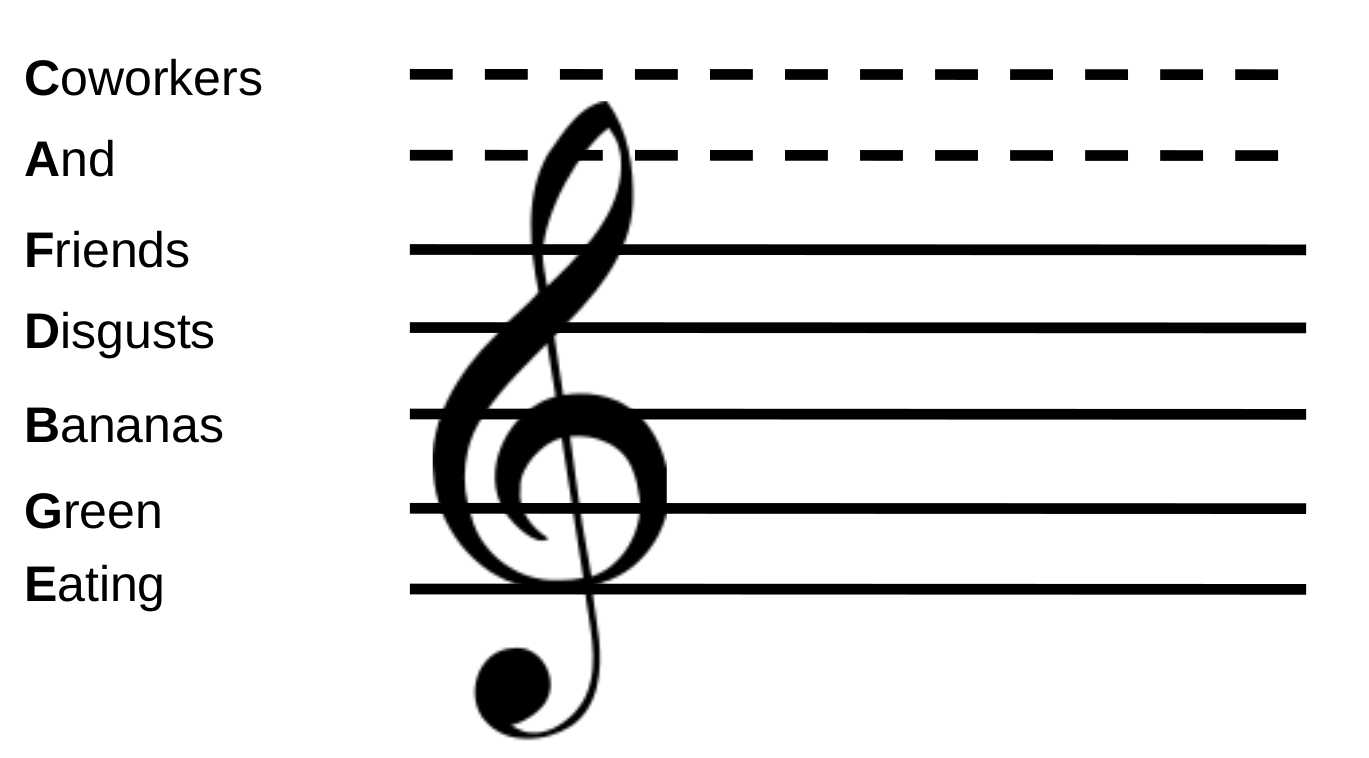
\includegraphics[width=8cm]{music-clef-mnemonic}
  };
  \draw[thick, ->] (0, -1.0) -- (10, -1.0) node[anchor=north east] {x (Время)};
  \draw[thick, ->] (0, -1.0) -- (0, 4.0) node[anchor=north east] {y (Частота)};
  \label{fig:lilypond-music-graph-1}
\end{tikzpicture}

Если читать слова снизу вверх, то образуется фраза ``\textbf{E}ating
\textbf{G}reen \textbf{B}ananas \textbf{D}isgusts \textbf{F}riends \textbf{A}nd
\textbf{C}oworkers'' (``Поедание зелёных бананов вызывает отвращение у друзей и
коллег по работе''). Первая буква слова кодирует ноту в научной нотации. Вверху
мы, помимо основных пяти линеек, подрисовали ещё две дополнительных линии,
выделив их пунктиром. На нотном стане дополнительные линии сверху и снизу
добавляются, если не хватает основных линий для записи композиции. Мнемоника
кодирует только основные линии нотного стана, однако зная их, мы можем понять,
какие ноты находятся между линиями.

%%%%%%%%%%%%%%%%%%%%%%%%%%%%%%%%%%%%%%%%%%%%%%%%%%%%%%%%%%%%%%%%%%%%%%%%%%%%%%%%
\section{Паузы в музыке}

Есть ещё один момент, на котором мы до текущего момента не заостряли внимание ---
паузы в произведении. Правильные паузы также важны, как и сами ноты.

В нотной записи паузы отмечаются специальными значками (см. рисунок
\ref{fig:lilypond-rest-example-1}.) \footnote{В музыке существуют паузы,
занммающие несколько тактов, либо очень короткие паузы -- тридцать вторые,
шестьдесят четвёртые и т.п. Используются они редко, поэтому мы их не будем
разбирать здесь.}

\begin{figure}[ht]
  \caption{Паузы в музыке.}
  \centering
  \begin{lilypond}
    \relative c' {
      \numericTimeSignature
      \time 4/4
      r1-"Целая."
    }
  \end{lilypond}
  \begin{lilypond}
    \relative c' {
      \numericTimeSignature
      \time 4/4
      r2-"Половинная." r2
    }
  \end{lilypond}
  \begin{lilypond}
    \relative c' {
      \numericTimeSignature
      \time 4/4
      r4-"Четвертная." r4 r4 r4
    }
  \end{lilypond}
  \begin{lilypond}
    \relative c' {
      \numericTimeSignature
      \time 4/4
      r8-"Восьмая." r8 r8 r8 r8 r8 r8 r8
    }
  \end{lilypond}
  \begin{lilypond}
    \relative c' {
      \numericTimeSignature
      \time 4/4
      r16-"Шестнадцатая." r16 r16 r16
      r16 r16 r16 r16
      r16 r16 r16 r16
      r16 r16 r16 r16
    }
  \end{lilypond}
  \label{fig:lilypond-rest-example-1}
\end{figure}

Целая пауза равна по длине целой ноте, половинная --- половине целой ноты и т.д.
Иными словами, мы можем использовать подход, примененный нами для высчитывания
длительности нот, для расчета длительности пауз в произведении.

Обозначения пауз с их длинтельностями предсавлены в таблице
\ref{table:music-rest-legths}.

\begin{table}[ht]
  \caption{Некоторые возможные длительности пауз.}
  \begin{tabular}{p{3cm}|p{4cm}|p{3.5cm}}
    Начертание & Длительность & Название \\
    \hline \hline
    \wholeNoteRest     & $\frac{1}{1}$ & ``Целая'' \\
    \hline
    \halfNoteRest      & $\frac{1}{2}$ & ``Половина'' \\
    \hline
    \crotchetRest        & $\frac{1}{4}$ & ``Четверть'' \\
    \hline
    \quaverRest    & $\frac{1}{8}$ & ``Восьмая'' \\
    \hline
    \semiquaverRest & $\frac{1}{16}$ & ``Шестнадцатая'' \\
    \hline
  \end{tabular}
  \label{table:music-rest-legths}
\end{table}

Для реализации паузы в программе необходимо во-первых создать специальную ноту с
нулевой частотой. Пауза в музыке называется ``Покой'' (или ``Rest''
по-английски), поэтому для обозначения паузы в программе мы будем использовать
заглавную букву ``R''.

\begin{verbatim}
const float R = 0; // Пауза ("Rest")
\end{verbatim}

Далее нам необходимо изменить функцию \texttt{play\_tone} таким образом, чтобы
она могла корректно ``воспроизводить'' паузы. Для этого нам необходимо добавить
такое условие, чтобы, если частота ноты больше нуля, то функция выполняла тот
код, который мы использовали раньше; иначе -- чтобы выполнялась просто задержка.

\begin{verbatim}
// Функция воспроизведения звука указанной частоты.
void play_tone(int port, float f, long t) {
  if (f > 0) {
    const int T = 1000000 / f;
    int d = T / 2;
    int count = t / T;
    for (int i = 0; i < count; i++) {
      digitalWrite(port, HIGH);
      delayMicroseconds(d);
      digitalWrite(port, LOW);
      delayMicroseconds(d);
    }
  } else {
    delay(t / 1000); // Пауза
  }
}
\end{verbatim}

Обратите внимание, что для создания задержки мы используем код \texttt{delay(t /
  1000)} -- делить \texttt{t} на 1000 необходимо по той причине, что время
проигрывания ноты (\texttt{t}) задаётся в микросекундах, а функция
\texttt{delay} принимает время ожидания в миллисекундах. Чтобы преобразовать
микросекунды в миллисекунды, достаточно поделить количество микросекунд на 1000
(так как в каждой микросекунде содержится 1000 миллисекунд.) Почему же мы не
могли использовать функцию \texttt{delayMicroseconds} для организации задержек
(пауз) прямо в микросекундах, без преобразования? Ответ прост --
\texttt{delayMicroseconds} не умеет долго ждать, и значения \texttt{t} для неё
будут слишком большими; если мы попытаемся использовать
\texttt{delayMicroseconds} с большими отрезками времени, то она не будет
корректно их обрабатывать, и задержка получится неправильной.

Для наглядной демонстрации использования пауз возьмём другое музыкальное
произведение -- ``Кабы небыло зимы'' из мультфильма ``Простоквашино''.

\begin{figure}[ht]
  \caption{Часть мелодии ``Кабы небыло зимы'' из мультфильма ``Простоквашино''.}
  \begin{lilypond}
    \relative c' {
      \key g \major
      \numericTimeSignature
      \time 4/4
      b8 b b'8. fis16 a8 g e4 |
      d8 d << b'8. d8. >> << c16 a >> << c8 a >> << b8 g8 >> r4
      d'8 c a fis << a c >> << g b >> << g4 b >>
      b,8 b << g'8. b8. >> << fis16 a >> << fis8 a >> << e8 g8 >> r4
    }
    \layout {
      indent = 0\mm
      line-width = 120\mm
      ragged-last = ##t
    }
  \end{lilypond}
  \label{fig:lilypond-melody-prostokvashino}
\end{figure}

В нотной записи на рисунке \ref{fig:lilypond-melody-prostokvashino} представлена
часть мелодии, которую мы попытаемся переложить на программный код. Полную
версию мелодии можно увидеть на рисунке
\ref{fig:lilypond-melody-prostokvashino-full}.

Можно заметить две четвертные паузы (\crotchetRest), которые необходимо добавить
в массив нот, чтобы произведение звучало, как в оригинале.

Можно также заметить двойные ноты, записанные одна над другой -- это значит, что
данные ноты должны играться одновременно. Для упрощения нашей задачи мы пока
будем брать самую верхнюю ноту из группы.

Попробуем вписать ноты в массив и послушать, как они будут звучать. Чтобы не
запутаться, разобъём ноты по группам, согласно тактам (по одной группе на
строке) -- а рядом с каждой группой в виде комментария напишем номер этого такта
(например, такт номер ноль мы пометили \texttt{/* 0 */}.)

\begin{verbatim}
float prostokvashino[28][2] = {
  /* 0 */ {b3, 8}, {b3, 8}, {b4, 8}, {f4, 16}, {a4, 8}, {g4, 8}, {e4, 4},
  /* 1 */ {d4, 8}, {d4, 8}, {d5, 8}, {c5, 16}, {c5, 8}, {b4, 8}, {R,  4},
  /* 2 */ {d5, 8}, {c5, 8}, {a4, 8}, {f4, 8},  {c5, 8}, {b4, 8}, {b4, 4},
  /* 3 */ {b3, 8}, {b3, 8}, {b4, 8}, {a4, 16}, {a4, 8}, {g4, 8}, {R,  4},
};
\end{verbatim}

При воспроизведении мелодия будет похожей на оригинал, однако вы можете заметить
некоторые ``несоответствия''. Источников данных несоответствий несколько. Первый
источник проблем в том, мы не учитываем, что длительность некоторых нот, которые
помечены точкой справа (вот так: ``\eighthNoteDotted'') больше стандартной.

%%%%%%%%%%%%%%%%%%%%%%%%%%%%%%%%%%%%%%%%%%%%%%%%%%%%%%%%%%%%%%%%%%%%%%%%%%%%%%%%
\section{Ноты с точками}

В музыкальной нотации точка, которая ставится справа от ноты, увеличивает её
длительность на половину от базовой.

Например, если у нас точка идёт после восьмушки (``\eighthNoteDotted''), то
следовательно к её длительности будет прибавляться половина от её длительности.
Половинка от восьмушки -- это шестнадцатая. Чтобы сложить простые дроби, которые
у нас получились, необходимо привести их к общему знаменателю. И формула
вычисления длительности будет следующая:

\begin{equation}
  \mbox{\eighthNoteDotted} = \mbox{\eighthNote} + \mbox{\sixteenthNote}
  = \frac{1}{8} + \frac{1}{16} = \frac{2}{16} + \frac{1}{16} = \frac{3}{16}
\end{equation}

Получившееся число $\frac{3}{16}$ для нас неудобно, так как мы в программе
подставляем в числитель дроби длительность одного такта, а тут у нас получается,
что необходимо поставить длину трёх тактов. Чтобы избавиться от этой неудобной
тройки в числителе, мы можем разделить числитель и знаменатель на 3.

\begin{equation}
  \frac{3 / 3}{16 / 3} = \frac{1}{16 / 3}
\end{equation}

Получившееся число $16 / 3$ необходимо подставить в массив с нашими нотами.
Например, третья нота нулевого такта -- ``B4'' -- как раз восьмая с точкой. В
массиве её длительность надо исправить -- вместо \texttt{\{b4, 8\}} написать
\texttt{\{b4, 16.0 / 3.0\}}. Тоже самое необходимо сделать с другими нотами,
возле которых стоит точка.

Для того, чтобы даннй код уместился в книгу, нам пришлось разбить каждый такт на
две строки, но по комментариям и отступам должно быть понятно, что происходит в
коде.

\begin{verbatim}
float prostokvashino[28][2] = {
  /* 0 */ {b3, 8},  {b3, 8}, {b4, 16.0 / 3.0},
  /*   */ {f4, 16}, {a4, 8}, {g4,          8}, {e4, 4},
  /* 1 */ {d4, 8},  {d4, 8}, {d5, 16.0 / 3.0},
  /*   */ {c5, 16}, {c5, 8}, {b4,          8}, {R,  4},
  /* 2 */ {d5, 8},  {c5, 8}, {a4,          8},
  /*   */ {f4, 8},  {c5, 8}, {b4,          8}, {b4, 4},
  /* 3 */ {b3, 8},  {b3, 8}, {b4, 16.0 / 3.0},
  /*   */ {a4, 16}, {a4, 8}, {g4,          8}, {R,  4},
};
\end{verbatim}

Теперь наша мелодия звучит ещё более похоже на оригинал.

Здесь стоит упомянуть, что в музыке встречаются ноты двумя точками справа, что
даёт удлинение ноты на половину её длительности и на половину от половины -- но
подобные ситуации редки из-за неудобства рассчёта необходимой длительности при
чтении музыкантом нот с листа. То ли дело нам, программистам -- прочитали
неспеша, запрограммировали, а там пусть компьютер сам пыжится над нашим
творением!

%%%%%%%%%%%%%%%%%%%%%%%%%%%%%%%%%%%%%%%%%%%%%%%%%%%%%%%%%%%%%%%%%%%%%%%%%%%%%%%%
\section{Полутона, диезы и бемоли}

Мы с вами всю эту главу говорим, что нот в октаве семь, и суммарно звуков 63
штуки, если считать по всем октавам. Но это не совсем точно -- на самом деле
звуков в октаве не семь, а двенадцать!

Вот так сюрприз. Откуда берутся дополнительные пять звуков? Оказывается, что в
музыке есть так называемые \emph{полутона}, которые позволяют разнообразить
музыку новыми звуками.

Нагляднее всего эти скрытные звуки легче всего увидеть на клавиатуре пианино.

\begin{figure}[ht]
  \caption{Одна октава на клавиатуре пианино.}
  \centering
  \begin{tikzpicture}
    \draw (0, 0) -- (7, 0);
    \foreach \x/\note in {0/C, 1/D, 2/E, 3/F, 4/G, 5/A, 6/B, 7/} {
      \draw (\x, 0) -- (\x, 2) -- (\x, 0) node[anchor=south west] {\note};
    };
    \foreach \x in {1, 2, 4, 5, 6} {
      \node[
        rectangle,
        draw,
        fill=black,
        minimum width=0.5cm,
        minimum height=1.35cm
      ] (r) at (\x, 1.30) {};
    };
  \end{tikzpicture}
  \label{fig:lilypond-music-graph-1}
\end{figure}

Видно, что между парами нот ``C''--``D'', ``D''--``E'', ``F''--``G'',
``G''--``A'', ``A''--``B'' находятся чёрные клавиши. Если мы посчитаем, сколько
всего клавиш в одной октаве, то получим двенадцать штук -- двенадцать звуков.

Объясняется это тем, что между двумя соседними клавишами \emph{расстояние в один
полутон}, если представить частотный диапазон октавы как некий отрезок.
Большинство пар нот имеют друг от друга достаточное расстояние, чтобы туда,
ровно посерёдке, добавить ещё одну клавишу (исключение составляют пары
``B''--``C'', ``E''--``F''.)

Каких-то особых закорючек для этих дополнительных звуков в музыке не
применяется, однако есть ``модификаторы'' для основных семи нот, поднимающих или
понижающих их частоту на полутон.

Для того, чтобы например получить частоту клавиши между парой ``C''--``D'',
можно поднять частоту ``C'' на пол-тона, либо понизить частоту ``D'' на те же
пол-тона.

Модификатор, повышающий частоту ноты на пол-тона называется \emph{диезом}, тогда
как аналогичный модификатор, понижающий частоту на пол-тона, называется
\emph{бемолем}.

Ноты с модификатором ``Диез'' помечаются решёткой (``\#''), стоящей перед нотой
-- например, на рис. \ref{fig:lilypond-f4-sharp} изображена ``Фа Диез''
четвёртой октавы.

\begin{figure}[ht]
  \caption{``Фа Диез'' четвёртой октавы.}
  \centering
  \begin{lilypond}
    \relative c' {
      \numericTimeSignature
      \time 4/4
      fis4
    }
  \end{lilypond}
  \label{fig:lilypond-f4-sharp}
\end{figure}

Чтобы высчитать частоту ``F4\#'', надо найти среднее арифметическое для частот
ноты ``F4'' и следующей перед ней ноты ``G4'' (см. формулу
\ref{quation:f-sharp-calculation}.)

\begin{equation}
  \frac{\mbox{F4} + \mbox{G4}}{2} = \mbox{F4\#}
  \label{quation:f-sharp-calculation}
\end{equation}

Программно вычислить ``F4\#'' не составляет труда, как показано в коде ниже.
Заметьте, что мы обозначили получившуюся частоту, как \texttt{f4s}, так как ``Фа
Диез'' по-английски пишется, как ``Fa Sharp'', и мы используем букву ``s'' из
слова ``sharp'' после ноты для краткости.

\begin{verbatim}
const float f4  = 349.230;
const float g4  = 392.000;
const float f4s = (f4 + g4) / 2; // F4 Диез
\end{verbatim}

Подобный подход работает и с другими нотами.

Кстати, для тех нот, после которых нет чёрной клавиши (``B'', ``E''), диезом
является просто следующая нота -- например, ``E4\#'' -- это ``F4'', а ``B4\#'' не
что иное, как ``C5''.

Таким образом:

\begin{verbatim}
const float e4  = 329.630;
const float f4  = 349.230;
const float e4s = f4; // E4 Диез
\end{verbatim}

Бемоли по логике работают схоже с диезами, с одним отличием -- они
\textbf{понижают} частоту ноты на половину тона. Обозначаются бемоли специальным
символом ``\flat'', который ставится перед нотой, на которую ``накладывается''
модификатор ``бемоль''.

Для примера возьмём ``E4\flat'' (см. рисунок \ref{fig:lilypond-e4-flat}.)

\begin{figure}[ht]
  \caption{``Фа Диез'' четвёртой октавы.}
  \centering
  \begin{lilypond}
    \relative c' {
      \numericTimeSignature
      \time 4/4
      ees4
    }
  \end{lilypond}
  \label{fig:lilypond-e4-flat}
\end{figure}

Бемоль для неё -- это частота ровно посерёдке между ``E4'' и предыдущей нотой от
неё (``D4''), как показано на формуле \ref{equation:e-flat-calculation}.

\begin{equation}
  \frac{\mbox{E4} + \mbox{D4}}{2} = \mbox{E4\flat}
  \label{equation:e-flat-calculation}
\end{equation}

Для обозначения бемолей в программном коде мы будем добавлять букву ``f'' к
имени ноты, после её номера октавы, так как в английском ноты с бемолями
называются ``приплюcнутыми'' (``flat'') -- например, ``E4 Бемоль'' будет
называться ``E4 Flat''.\footnote{В музыке иногда встречатеся двойные диезы и
двойные бемоли, что означает необходимость брать ноту на два полутона выше или
ниже -- по сути, брать следующую или предыдующую ноту.}

\begin{verbatim}
const float d4  = 293.660;
const float e4  = 329.630;
const float e4f = (e4 + d4) / 2; // E4 Бемоль
\end{verbatim}

Все эти диезы и бемоли мы пока с вами рассматривали в вариантах, когда
знак-модификатор пишется разу перед нотой, на которую ``накладывается
заклинание'' -- они называются знаками ``по-месту'', или ``случайными'' (англ.
\emph{accidentals}.) Но музыкантам неудобно писать подобные модификаторы перед
каждой нотой, если подобных случаев в композиции много. Чтобы решить эту
проблему, в музыке используются знаки диезов и бемолей, которые ставятся в
начале нотного стана -- в начале линий нотоносца. Влияние таких значков
распространяется на все ноты подобные той, на которую наложено ``заклинание''.

Вернёмся к мелодии ``Кабы небыло зимы''.  Если посмотреть на начало каждой
строки, то можно увидеть решёнку на ``F5'' -- это означает, что все ноты ``F''
будут диезами.

\begin{tikzpicture}
  \node (image) at (4, 0) {
    \begin{lilypond}
      \relative c' {
        \key g \major
        \numericTimeSignature
        \time 4/4
        b8 b b'8. fis16 a8 g e4 |
        d8 d << b'8. d8. >> << c16 a >> << c8 a >> << b8 g8 >> r4
      }
      \layout {
        indent = 0\mm
        line-width = 120\mm
        ragged-last = ##t
      }
    \end{lilypond}
  };
  \draw[red, thick, ->] (0.0, 1.0) node[anchor=south west] {F5 Диез} -- (-0.5, 0.5);
  \label{fig:lilypond-melody-prostokvashino-2}
\end{tikzpicture}

Зная это, мы можем соответствующим образом модифицировать код нашей мелодии.

\begin{verbatim}
const float f4s = (f4 + g4) / 2;

// ...

float prostokvashino[28][2] = {
  /* 0 */ {b3,  8},  {b3, 8}, {b4, 16.0 / 3.0},
  /*   */ {f4s, 16}, {a4, 8}, {g4,          8}, {e4, 4},
  /* 1 */ {d4,  8},  {d4, 8}, {d5, 16.0 / 3.0},
  /*   */ {c5,  16}, {c5, 8}, {b4,          8}, {R,  4},
  /* 2 */ {d5,  8},  {c5, 8}, {a4,          8},
  /*   */ {f4s, 8},  {c5, 8}, {b4,          8}, {b4, 4},
  /* 3 */ {b3,  8},  {b3, 8}, {b4, 16.0 / 3.0},
  /*   */ {a4,  16}, {a4, 8}, {g4,          8}, {R,  4},
};

// ...
\end{verbatim}

%%%%%%%%%%%%%%%%%%%%%%%%%%%%%%%%%%%%%%%%%%%%%%%%%%%%%%%%%%%%%%%%%%%%%%%%%%%%%%%%
\section{Музыкальный размер}

Вы могли видеть, что на нотном стане в самом начале, возле скрипичного (или
басового) ключа часто написано $\frac{4}{4}$ -- что же это означает?

Пометка $\frac{4}{4}$ (читается как ``четыре четверти'') обозначает
\emph{музыкальный размер} произведения.  С точки зрения кодирования мелодии в
программе это не влияет ни на частоту нот, ни на их длительность.  При этом,
однако, данная пометка напрямую влияет на звучание произведения, и без её учёта
все произведения будут звучать ``плоско'' и менее интересно.

Удивительный эффект музыкальнй размер даёт благодаря \emph{акцентированию}
определённых нот.

Например, посмотрим ещё раз на ``Twinkle, Twinkle, Little Star''
(\ref{fig:lilypond-musical-scale-example-1}.)

\begin{figure}[ht]
  \caption{``Twinkle, Twinkle, Little Star'' в размере четыре четверти.}
  \centering
  \begin{lilypond}
    \relative c' {
      \numericTimeSignature
      \time 4/4
      c4 c g' g
      a a g2
      f4 f e e
      d d c2
      g'4 g f f
      e e d2
      g4 g f f
      e e d2
      c4 c g' g
      a a g2
      f4 f e e
      d d c2
    }
    \layout {
      indent = 0\mm
      line-width = 100\mm
      ragged-last = ##t
    }
  \end{lilypond}
  \label{fig:lilypond-musical-scale-example-1}
\end{figure}

Поскольку композиция записана в музыкальном размере ``четыре четверти'', то в
один такт убирается ровно четыре четвёртных ноты, или суммарно единица (или одна
целая нота.)  Числитель данной дроби указывает, сколько частей -- или, по-другому
называемые \emph{долей} -- убирается в такт.  Знаменатель дроби указывает, на
какие именно доли делится такт.  В размере ``четыре четверти'' такт делится на
четыре части по одной четвертной ноте.

При игре музыкального произведения на каком-либо инструменте акцент идёт обычно
на первую ноту из такта -- на её \emph{сильную долю}.  Доли, которые не
акцентированы, называются \emph{слабыми долями}.

С точки зрения исполнения акцентированные ноты должны звучать громче, или
каким-либо другим способом выделяться в общем звучании.

Акцент нот обозначается значком ``>'' над (или под) нотой.  Если мы расставим
значки, обозначающие акцент, то получим следующую запись
(см. рис. \ref{fig:lilypond-musical-scale-example-2}.)

\begin{figure}[ht]
  \caption{``Twinkle, Twinkle, Little Star''}
  \centering
  \begin{lilypond}
    \relative c' {
      \numericTimeSignature
      \time 4/4
      c4-> c g'-> g
      a-> a g2->
      f4-> f e->  e
      d-> d c2->
      g'4-> g f-> f
      e-> e d2->
      g4-> g f-> f
      e-> e d2->
      c4-> c g'-> g
      a-> a g2->
      f4-> f e-> e
      d-> d c2->
    }
    \layout {
      indent = 0\mm
      line-width = 100\mm
      ragged-last = ##t
    }
  \end{lilypond}
  \label{fig:lilypond-musical-scale-example-2}
\end{figure}

Музыкальный размер ``четыре четверти'' называется \emph{сложным}, так как он
получен слиянием двух более \emph{простых} размеров, а именно ``две четверти''.

Таким образом, в размере ``четыре четверти'' кроме сильной доли, появляется
вторая доля, называемая \emph{относительно сильной}.

Как можно видеть на рис. \ref{fig:lilypond-musical-scale-example-2}, первый
(основной) акцент ставится на первую ноту в такте -- в нашем случае, первую
четверть.  Второй, второстепенный, акцент ставится на третью ноту в такте, или
же можно сказать, что на первую ноту второй половины такта (относительно сильную
долю.)  Основной акцент по определению более выраженный, чем второстепенный.

Если мы возьмём другой музыкальный размер -- например, две четверти
($\frac{2}{4}$), то произведение будет звучать по-другому, поскольку основной и
единственный акцент будет на первую ноту каждого такта, и относительно слабая
доля будет отстуствовать.

\begin{figure}[ht]
  \caption{``Twinkle, Twinkle, Little Star'' в размере две четверти.}
  \centering
  \begin{lilypond}
    \relative c' {
      \numericTimeSignature
      \time 2/4
      c4-> c
      g'-> g
      a-> a
      g2->
      f4-> f e->  e
      d-> d c2->
      g'4-> g f-> f
      e-> e d2->
      g4-> g f-> f
      e-> e d2->
      c4-> c g'-> g
      a-> a g2->
      f4-> f e-> e
      d-> d c2->
    }
    \layout {
      indent = 0\mm
      line-width = 100\mm
      ragged-last = ##t
    }
  \end{lilypond}
  \label{fig:lilypond-musical-scale-example-3}
\end{figure}

Музыкальный размер ``две четверти'' используется в таких стилях музыки, как
например полька.

Если мы возьмём музыкальный размер ``три четверти''
(см. рис. \ref{fig:lilypond-musical-scale-example-4}), в такт будет убираться
ровно три четвертных ноты.  Таким образом, акцент будет идти на первую четверть
из трёх в каждом такте.  При этом, некоторые ноты длиной $\frac{1}{2}$ как бы
``разрезаются'' тактовой чертой на две четверти.

\begin{figure}[ht]
  \caption{``Twinkle, Twinkle, Little Star'' в размере три четверти}
  \centering
  \begin{lilypond}
    \relative c' {
      \numericTimeSignature
      \time 3/4
      c4->  c g'
      g->   a a
      g2->  f4
      f->   e e
      d->   d c4~4->
      g'4   g
      f->   f e
      e->   d2
      g4->  g f
      f->   e e
      d2    c4
      c->   g' g
      a->   a g4~4->
      f4    f
      e->   e d
      d->   c2
    }
    \layout {
      indent = 0\mm
      line-width = 100\mm
      ragged-last = ##t
    }
  \end{lilypond}
  \label{fig:lilypond-musical-scale-example-4}
\end{figure}

Такая запись в отношении ``Twinkle, Twinkle, Little Star'' выглядит
противоестественно, и после таких экспериментов к вам в дверь может постучатся
музыкальная инквизиция.

Тем не менее, если мы сыграем в таком размере композицию музыкальном
инструменте, то она будет звучать вальсирующе, ведь музыкальнй размер ``две
четверти'' обычно используется для вальса.

Каким же образом мы можем выразить эти музыкальные нюансы в нашем программном
коде и в реализации аппаратной части, чтобы они украсили наше музыкальное
произведение?  Изменение кода включает в себя несколько этапов.

Во-первых, самым простым для нас способом выделить какие-то определённые ноты
является подключение дополнительного динамика с меньшей громкостью к Arduino.
Ноты, которые должны звучать тише, будут отправляться на него.  А те ноты,
которые должны быть акценированными, будут отправлятсья на громкий динамик.
Допустим, громкий динамик будет у нас на цифровом порту 2, а тихий динамик -- на
цифровом порту 3.

\begin{verbatim}
const int LOUD_SPEAKER_PIN  = 2; // Громкий динамик.
const int QUIET_SPEAKER_PIN = 3; // Тихий динамик.

// ...

void setup() {
  pinMode(LOUD_SPEAKER_PIN, OUTPUT);
  pinMode(QUIET_SPEAKER_PIN, OUTPUT);
}
\end{verbatim}

Во-вторых, двумерный массив нот должен теперь иметь не два столбца, а три, так
как в третьем столбце мы как раз будем хранить громкость ноты.  Исходя из
параметра громкости, который на данный момент может иметь всего два уровня -- 0
(тихо) и 1 (громко), мы будем выбирать динамик для воспроизведения ноты.

Для размера ``четыре четверти'' мы будем первую ноту из такта делать громче
остальных.

\begin{verbatim}
// ...

float twinkle_twinkle_little_star[][3] = {
  /* 0 */ {c4, 4, 1}, {c4, 4, 0}, {g4, 4, 0}, {g4, 4, 0},
  /* 1 */ {a4, 4, 1}, {a4, 4, 0}, {g4, 4, 0},
  /* 2 */ {f4, 4, 1}, {f4, 4, 0}, {e4, 4, 0}, {e4, 4, 0},
  /* 3 */ {d4, 4, 1}, {d4, 4, 0}, {c4, 4, 0},

  /* 4 */ {g4, 4, 1}, {g4, 4, 0}, {f4, 4, 0}, {f4, 4, 0},
  /* 5 */ {e4, 4, 1}, {e4, 4, 0}, {d4, 4, 0},
  /* 6 */ {g4, 4, 1}, {g4, 4, 0}, {f4, 4, 0}, {f4, 4, 0},
  /* 7 */ {e4, 4, 1}, {e4, 4, 0}, {d4, 4, 0},

  /* 4 */ {c4, 4, 1}, {c4, 4, 0}, {g4, 4, 0}, {g4, 4, 0},
  /* 5 */ {a4, 4, 1}, {a4, 4, 0}, {g4, 4, 0},
  /* 2 */ {f4, 4, 1}, {f4, 4, 0}, {e4, 4, 0}, {e4, 4, 0},
  /* 3 */ {d4, 4, 1}, {d4, 4, 0}, {c4, 4, 0},
};

// ...
\end{verbatim}

Далее при воспроизведении музыки нам надо выбирать нужный динамик, в
соответствии с громкостью (акцентом) ноты.

\begin{verbatim}
// ...

void loop() {
  const long BPM = 120;
  const long MINUTE = 60 * 1000000;
  const long T = (MINUTE / BPM) * 4;

  for (int note_idx = 0; note_idx < 28; note_idx++) {
    if (melody[note_idx][2] == 1) {
      // Нота с акцентом
      play_tone(LOUD_SPEAKER_PIN,
                melody[note_idx][0],
                T / melody[note_idx][1]);
    } else {
      // Нота без акцента
      play_tone(QUIET_SPEAKER_PIN,
                melody[note_idx][0],
                T / melody[note_idx][1]);
    }
    delay(100);
  }
}
\end{verbatim}

%%%%%%%%%%%%%%%%%%%%%%%%%%%%%%%%%%%%%%%%%%%%%%%%%%%%%%%%%%%%%%%%%%%%%%%%%%%%%%%%
\section{Басовый ключ}

Кроме скрипичного ключа в музыке часто используется \emph{басовый ключ}.  Обычно
басовый ключ используется для тех музыкальных инструментов, у которых частотный
диапазон находится ниже, чем охватывает скрипичный ключ.

Мнемоника для басового ключа представлена на
рис. \ref{fig:lilypond-music-graph-2}.

\begin{figure}[ht]
  \caption{Мнемоника для запоминания нот басового ключа.}
  \begin{tikzpicture}
    \node (image) at (4, 2) {
      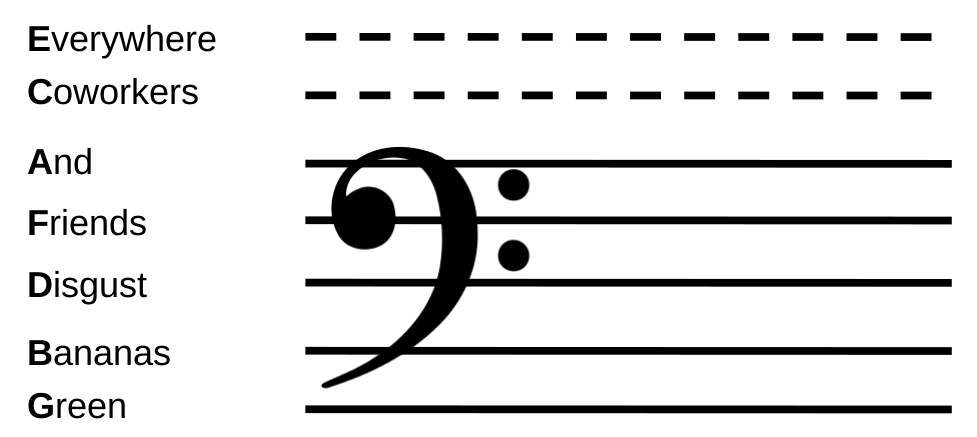
\includegraphics[width=8cm]{music-bass-clef-mnemonic}
    };
    \draw[thick, ->] (0, -1.0) -- (10, -1.0) node[anchor=north east] {x (Время)};
    \draw[thick, ->] (0, -1.0) -- (0, 4.0) node[anchor=north east] {y (Частота)};
  \end{tikzpicture}
  \label{fig:lilypond-music-graph-2}
\end{figure}

%%%%%%%%%%%%%%%%%%%%%%%%%%%%%%%%%%%%%%%%%%%%%%%%%%%%%%%%%%%%%%%%%%%%%%%%%%%%%%%%
\chapter{Приложения}

\section{Приложение А}
\label{section:appendixA}
\begin{longtable}{crll}
  № октавы & Слоговое обозначение & Научное обознечение & Частота (Гц) \\
  \hline \hline

  \multirow{7}{*}{0}
  \musicnote{0}{C}{16.352}
  \cline{2-4}
  \musicnote{0}{D}{18.354}
  \cline{2-4}
  \musicnote{0}{E}{20.602}
  \cline{2-4}
  \musicnote{0}{F}{21.827}
  \cline{2-4}
  \musicnote{0}{G}{24.500}
  \cline{2-4}
  \musicnote{0}{A}{27.500}
  \cline{2-4}
  \musicnote{0}{B}{30.868}
  \hline

  \multirow{7}{*}{1}
  \musicnote{1}{C}{32.703}
  \cline{2-4}
  \musicnote{1}{D}{36.708}
  \cline{2-4}
  \musicnote{1}{E}{41.203}
  \cline{2-4}
  \musicnote{1}{F}{43.654}
  \cline{2-4}
  \musicnote{1}{G}{48.999}
  \cline{2-4}
  \musicnote{1}{A}{55.000}
  \cline{2-4}
  \musicnote{1}{B}{61.735}
  \hline

  \multirow{7}{*}{2}
  \musicnote{2}{C}{65.406}
  \cline{2-4}
  \musicnote{2}{D}{73.416}
  \cline{2-4}
  \musicnote{2}{E}{82.407}
  \cline{2-4}
  \musicnote{2}{F}{87.307}
  \cline{2-4}
  \musicnote{2}{G}{97.999}
  \cline{2-4}
  \musicnote{2}{A}{110.000}
  \cline{2-4}
  \musicnote{2}{B}{123.470}
  \hline

  \multirow{7}{*}{3}
  \musicnote{3}{C}{130.810}
  \cline{2-4}
  \musicnote{3}{D}{146.830}
  \cline{2-4}
  \musicnote{3}{E}{164.810}
  \cline{2-4}
  \musicnote{3}{F}{174.610}
  \cline{2-4}
  \musicnote{3}{G}{196.000}
  \cline{2-4}
  \musicnote{3}{A}{220.000}
  \cline{2-4}
  \musicnote{3}{B}{246.940}
  \hline

  \multirow{7}{*}{4}
  \musicnote{4}{C}{261.630}
  \cline{2-4}
  \musicnote{4}{D}{293.660}
  \cline{2-4}
  \musicnote{4}{E}{329.630}
  \cline{2-4}
  \musicnote{4}{F}{349.230}
  \cline{2-4}
  \musicnote{4}{G}{392.000}
  \cline{2-4}
  \musicnote{4}{A}{440.000}
  \cline{2-4}
  \musicnote{4}{B}{493.880}
  \hline

  \multirow{7}{*}{5}
  \musicnote{5}{C}{523.250}
  \cline{2-4}
  \musicnote{5}{D}{587.320}
  \cline{2-4}
  \musicnote{5}{E}{659.260}
  \cline{2-4}
  \musicnote{5}{F}{698.460}
  \cline{2-4}
  \musicnote{5}{G}{783.990}
  \cline{2-4}
  \musicnote{5}{A}{880.000}
  \cline{2-4}
  \musicnote{5}{B}{987.770}
  \hline

  \multirow{7}{*}{6}
  \musicnote{6}{C}{1046.500}
  \cline{2-4}
  \musicnote{6}{D}{1174.700}
  \cline{2-4}
  \musicnote{6}{E}{1318.500}
  \cline{2-4}
  \musicnote{6}{F}{1396.900}
  \cline{2-4}
  \musicnote{6}{G}{1568.000}
  \cline{2-4}
  \musicnote{6}{A}{1760.000}
  \cline{2-4}
  \musicnote{6}{B}{1975.500}
  \hline

  \multirow{7}{*}{7}
  \musicnote{7}{C}{2093.000}
  \cline{2-4}
  \musicnote{7}{D}{2349.300}
  \cline{2-4}
  \musicnote{7}{E}{2637.000}
  \cline{2-4}
  \musicnote{7}{F}{2793.800}
  \cline{2-4}
  \musicnote{7}{G}{3136.000}
  \cline{2-4}
  \musicnote{7}{A}{3520.000}
  \cline{2-4}
  \musicnote{7}{B}{3951.100}
  \hline

  \multirow{7}{*}{8}
  \musicnote{8}{C}{4186.000}
  \cline{2-4}
  \musicnote{8}{D}{4698.600}
  \cline{2-4}
  \musicnote{8}{E}{5274.000}
  \cline{2-4}
  \musicnote{8}{F}{5587.700}
  \cline{2-4}
  \musicnote{8}{G}{6271.900}
  \cline{2-4}
  \musicnote{8}{A}{7040.000}
  \cline{2-4}
  \musicnote{8}{B}{7902.100}
  \hline

  \caption{Октавная система}
  \label{table:octaveList}

\end{longtable}

\newpage
\section{Приложение Б}

\begin{figure}[ht]
  \caption{Мелодия ``Кабы небыло зимы'' из мультфильма ``Простоквашино''.}
  \begin{lilypond}
    \relative c' {
      \key g \major
      \numericTimeSignature
      \time 4/4
      %% 0
      (b'8 b cis dis e4-.) << g,8 b e >> r8 \bar ".|:"
      %% 1
      b,8 b b'8. fis16 a8 g e4 |
      %% 2
      d8 d << b'8. d8. >> << c16 a >> << c8 a >> << b8 g8 >> r4
      %% 3
      d'8 c a fis << a c >> << g b >> << g4 b >>
      %% 4
      b,8 b << g'8. b8. >> << fis16 a >> << fis8 a >> << e8 g8 >> r4
      %% 5
      b,8 b b'8. fis16 a8 g8 e4
      %% 6
      d8 d << b'8. d8. >> << a16 c >> << a8 c >> << g8 b8 >> r8 e4
      %% 7
%%       e8)
%%       d8 d
    }
    \layout {
      indent = 0\mm
      line-width = 120\mm
      ragged-last = ##t
    }
  \end{lilypond}
  \label{fig:lilypond-melody-prostokvashino-full}
\end{figure}


\section{Список сокращений}
\begin{acronym}
  \acro{ШИМ}{Широтно-импульсная модуляция}
\end{acronym}
\end{document}

